\chapter{Macrosegregation with solidification shrinkage}
%\chaptermark{Nonlinear Temperature Solver}
\begin{nolinkcolors} 
\minitoc
\end{nolinkcolors}
\newpage

% ======================
\section{Solidification shrinkage}
% ======================

Solidification shrinkage is, by definition, the effect of relative density change between the liquid and solid phases.
In general, it results in a progressive volume change during solidification, until the phase change has finished. 
The four stages in \cref{fig:real_ingot_stage_a,fig:real_ingot_stage_c,fig:real_ingot_stage_b,fig:real_ingot_stage_d} depict the volume change with 
respect to solidification time.
First, at the level of the first solid crust, near the local solidus temperature, the solid forms with a density greater than 
the liquid's. The subsequent volume decrease creates voids with a negative pressure, forcing the fluid to be sucked in the direction of the volume change 
(cf. \cref{fig:real_ingot_stage_b}). As a direct result of the inward feeding flow, the ingot surface
tends to gradually deform in the feeding direction, forming the so-called \emph{shrinkage pipe}, shown in \cref{fig:shrinkage_exp}. 
Since the mass of the alloy and its chemical species is conserved, 
a density difference between the phases ($\rhol < \rhos \implies \frac{\rhol}{\rhos}<1$) eventually leads 
to a different overall volume ($V^s<V^l$) once solidification is complete, as confirm the following equations:
%------------
\begin{subequations}
\begin{align}
& \rhol V^l = \rhos V^s  \\ 
& V^s = \frac{\rhol}{\rhos} V^l
\end{align}
\end{subequations}
%------------
Solidification shrinkage is not the only factor responsible for volume decrease. 
Thermal shrinkage in both solid and liquid phases, as well 
as solutal shrinkage in the liquid phase are also common causes in a casting process. 
However, thermal shrinkage is very important to apprehend, as temperature decreases in steel casting, usually exceeding a \SI{1000}{\udegC}, thus causing substantial density variations. 
%Henceforth, we will focus on shrinkage due to phase change.
%
%Talk and explain models in the literature that predict shrinkage (without or with macrosegregation): Beckermann, Wu ? \\
%Show and comment the experiments that have been done: Hebditch and Hunt, Smacs Hachani  ...
%
%\comment{ \textbf{Sutaria2012} talk about feeding paths, but more importantly they computed thermal shrinkage WITHOUT solving
%NavierStokes equations. To predict the interface shape, they solve a LS transport with an imposed velocity given by Gada et Sharma 2009}
%
%
%----------------
%
\begin{figure}[htbp]
\centering
%\begin{minipage}{.5\textwidth}
  \begin{subfigure}{0.3\textwidth}
    \centering
    \def\svgwidth{100pt}
	\import{Chapter4/Graphics/new/}{ingot_air_liq.pdf_tex}
	\caption{Initial state}
    \label{fig:real_ingot_stage_a}
  \end{subfigure}
  %\hfill
  \begin{subfigure}{0.3\textwidth}
    \centering
    \def\svgwidth{100pt}
	\import{Chapter4/Graphics/new/}{ingot_air_liq_mush_sol.pdf_tex} 
	\caption{Early intermediate state}
    \label{fig:real_ingot_stage_b}
  \end{subfigure}
%
\vskip\baselineskip
%======
%
  \begin{subfigure}{0.3\textwidth}
    \centering
    \def\svgwidth{100pt}
	\import{Chapter4/Graphics/new/}{ingot_air_mush_sol.pdf_tex}
	\caption{Late intermediate state}
    \label{fig:real_ingot_stage_c}
  \end{subfigure}
  %\hfill
  \begin{subfigure}{0.3\textwidth}
    \centering
    \def\svgwidth{100pt}
	\import{Chapter4/Graphics/new/}{ingot_air_sol.pdf_tex}
	\caption{Final state}
    \label{fig:real_ingot_stage_d}
  \end{subfigure}
  %
\caption{Schematic of the main cooling stages of an ingot against side and bottom mould walls (not shown)}
\label{fig:real_ingot_stages}
\end{figure}
%
%---------------------
%
%----------------------
\begin{figureth}
% textwidth 
{0.45}
%path 
{Chapter4/Graphics/shrinkage_exp.png}
% caption
{Sulphur prints of three ingots showing pipe formation at the top as a result 
of solidification shrinkage with various ingot inclination during casting \citep{onodera_effect_1959}.
Positive macrosegregation is clearly seen in this area, while A-shape and V-shape positive mesosegregates are detected
at the ingot's tips and center respectively.}
% label
\label{fig:shrinkage_exp}
\end{figureth}
%-----------------------------------
%
%
%============================================
\section{Choice of interface tracking}
%============================================
In chapter 2, several methods of interface tracking/capturing methods were presented 
along with their similarities and differences. In the case of solidification shrinkage,
the metal-air interface can be tracked with any method from the previously mentioned.
However, several reasons motivate us to settle on the level set method. 
First, the easiest solution is testing a method which already exists in \cimlib library.
The level set method was implemented by HERE as a framework for monolithic resolution. Since this work,
the method has been extensively used and improved in several projects mainly for multiphase flows, which is the 
main competence of the Computing and FLuids (C.F.L) group at CEMEF. Another motivation is the compatibility
between \cimlib and \thercast, where the latter is the final destination of the code developed during for the Ph.D. thesis.
In its recent versions, \thercast handles laminar and turbulent ingot filling where the level set method is used 
to capture the free surface of the molten metal. Aside from the practical motivations, some technical aspects of the level
set method make it very attractive to apply it macroscopic surface tracking (in contrast to microscopic interface tracking, 
for instance the solid-liquid interface), such as topological properties that are readily available (e.g. curvature)
and accurate position compared to volume-based methods like VOF.
%
%============================================
\section{Multidomain formalism}
%============================================
In the previous chapters, we considered in our simulations the metal as a 
saturated mixture of solid and liquid during solidification.
It means that no gas phase may appear during the process, and this  this chapter.
The reason is we chose to describe our model in Eulerian description, 
for which we have considered a fixed grid to discretise the averaged conservation 
equations governing the phase change between the liquid and solid phases.
Furthermore, with the introduction of shrinkage, an increase in global density means 
that a gas phase should enter the domain to replace the shrunk volume.
At this point, several interfaces may be distinguished: liquid-solid ($l$-$s$), liquid-air ($l$-$a$) and solid-air ($s$-$a$), where 
we defined 2 phases ($l$ and $s$) belonging to the "Metal" domain denoted $M$, while the "Air" domain, denoted $A$, 
is made up of a unique phase, ($a$), with the same name. As a standard for this formalism, we consider that uppercase letters
are used for domains, while lowercase letters are used for phases.

The main idea behind the multidomain formalism, is to go from the classic 
conservations equations introduced by  volume averaging in chapter 2,
in the context of a solidifying two-phase system to generalise it by taking
into account a third gas phase, such as:
%-------------
\begin{align}
\label{eq:}
V^l + V^s + V^a = \rev \\
\gl + \gs + \ga = 1
\end{align} 
%-------------
while keeping a physical integrity with the former monodomain model. 
Then, one is free to choose a suitable numerical method to track the 
interfaces between the several phases. In our applications, we are particularly 
interested in keeping an indirect representation of the $l$-$s$ interface (dotted line in \cref{fig:rev_triphase})
using the volume averaging theory, while employing a different
method to track the $l$-$a$ and $s$-$a$ interfaces (dashed lines in \cref{fig:rev_triphase}) with the level set method. 
This allows switching to the latter method in a physically representative manner.

In this context, each domain can be seen as a material having a physical
interface with the other domains. As a consequence of our interpretation, 
the gas phase should not exist in the metal, which may naturally
occur if the thermodynamic conditions are in favour of nucleating and growing 
a new phase, or in the case of a gas that was trapped inside mould grooves.
%----------------------
\begin{figureth}
% textwidth 
{0.45}
%path 
{Chapter4/Graphics/REV_triphase.pdf}
% caption
{Schematic of a representative volume element containing 3 phases with distinct velocities, separated by 3 interfaces.
The dotted line is the indirectly tracked solid-liquid interface while the other dashed lines, air-liquid and air-solid
interfaces, are directly tracked.}
% label
\label{fig:rev_triphase}
\end{figureth}
%-----------------------------------
%
%
%------------
\subsection{Assumptions}
%------------
Each phase in the system has its own velocity, $\vl$, $\vs$ and $\va$, while the respective
interfaces $\liqsol$, $\liqair$ and $\solair$ have different and independent velocities, 
represented by $\vliqsol$, $\vliqair$ and $\vsolair$. Note that the solid-liquid interface
velocity was denoted $\vstar$ in the previous chapters as no more than two phases were considered.
The first major assumption is that the solid phase, once formed from the liquid, is fixed and rigid.
It means that no subsequent deformation may occur and therefore $\vsolair$ reduces to vector zero.
Moreover, we use the already introduced volume averaging principles to write locally for any quantity $\psi$:
%------------
\begin{subequations}
\begin{align}
\label{eq:}
\avg{\psi} &= \avg{\psi^l} + \avg{\psi^s} + \avg{\psi^a} \\
			&= \gl \psi^l + \gs \psi^s  + \ga \psi^a
\end{align}
\end{subequations}
%------------
where volume fractions, $\gphi$, for each phase $\phi$ were used. \citet{rappaz_numerical_2003} define
the volume fraction by writing a general expression inside the representative volume $\rev$:
%------------
%\begin{subequations}
\begin{align}
\label{eq:}
\gphi = \frac{1}{\rev} \integral{\rev}{\chi^\phi(x,t)}{\Ohm} = \avg{\chi^\phi}
\end{align}
%\end{subequations}
%------------
where the integrated quantity is an indicator (or presence) function relative to phase $\phi$, which
defines the volume of this phase in the system, $\Ohm^\phi$, as follows:
%------------
%\begin{subequations}
\begin{align}
\label{eq:}
\chi^\phi(x,t)=
\begin{cases}
  1 	& \text{ if } x \in \Ohm^\phi \\ 
  0 	& \text{otherwise}
\end{cases}
\end{align}
%\end{subequations}
%------------
Any phenomenon that may displace an interface, whether by phase change or a phase motion, is 
mathematically translated by variations of the presence function, such that its total derivative for each phase
satisfies the following:
%
%------------
\begin{align}
\label{eq:transport_presence}
& \frac{d \chi^\phi}{dt} = \tempup{\chi^\phi} + \vstar \cdot \nabvec \chi^\phi = 0
\end{align}
%------------
%
If we consider the liquid phase, the variations of any quantity, named $\psi$, are given by:
%------------
\begin{align}
\label{eq:}
& \avg{{\tempup{\psi^l}}} = \tempup{\avg{\psi^l}}
							- \frac{1}{\rev} \integral{l-a}{\psi^l \vliqair \cdot \nliqair}{\Gamma}
							- \frac{1}{\rev} \integral{l-s}{\psi^l \vliqsol \cdot \nliqsol}{\Gamma} \\
& \avg{\nabvec \psi^l} =  \nabvec{\avg{\psi^l}} 
							+ \frac{1}{\rev} \integral{l-a}{\psi^l \nliqair}{\Gamma} 
							+\frac{1}{\rev} \integral{l-s}{\psi^l \nliqsol }{\Gamma} \\
& \avg{\nabvec \cdot \vec{\psi}^l} =  \nabvec \cdot {\avg{\vec{\psi}^l}} 
							+ \frac{1}{\rev} \integral{l-a}{\vec{\psi^l} \cdot \nliqair }{\Gamma} 
							+\frac{1}{\rev} \integral{l-s}{\vec{\psi^l} \cdot  \nliqsol }{\Gamma}							
\end{align}
%------------
\Cref{eq:transport_presence} can be recast with the level set method by using the smoothed Heaviside function in the metal.
For the metal, this function is equal to one and decreases to zero in the air in a smooth way across both interfaces, solid-air and liquid-air.
Since the solid phase is assumed fixed without possible deformation, and knowing that air is assumed incompressible, 
the solid-air interface does not move, leading to the following equation: 
%------------
\begin{align}
\label{eq:transport_heaviside}
& \frac{d \heavisideM}{dt} = \tempup{\heavisideM} + \vliqair \cdot \nabvec \heavisideM = 0
\end{align}
%------------
%======================
\section{FE partitioned model}
%--------------------------------------------------
%
In this section, we start from a the monodomain finite element model 
presented in \cref{sec:monodomain} that was relevant to the metal only, 
referred to by the superscript $M$, then present the essential assumptions and formulations 
that allow predicting solidification shrinkage in a Eulerian context that introduces
another domain, the air, referred to by the superscript $A$.
\subsection{In the metal}
%
\subsubsection{Mass and momentum conservation}
By assuming a fixed solid phase ($\vs=\vec{0}$), the average velocity in the metal reduces only to liquid's average velocity.
Therefore, we can write:
%------------
\begin{align}
\label{eq:vitmetal}
& \vM = \vit = \gl \vl 
\end{align}
%------------
With \cref{eq:vitmetal}, the mass balance in the metal writes:
%------------
\begin{subequations}
\begin{align}
& \tempup{\avg{\rho}^M} + \nabla \cdot \avg{\rho \vec{v}}^M  = 0 \\ 
& \tempup{\avg{\rho}^M} + \nabla \cdot \brac{ \gl \rhol \vl} = 0 \\ 
& \tempup{\avg{\rho}^M} + \rhol \nabla \cdot \brac{ \gl \vl} 
	+ \gl \vl \cdot  \nabvec \rhol = 0 \\	
\label{eq:mass_balance_metal}
& \nabla \cdot \vit 
= -\frac{1}{\rhol} \brac{\tempup{\avg{\rho}^M }+ \vit \cdot  \nabvec \rhol}
\end{align}
\end{subequations}
%------------
\Cref{eq:mass_balance_metal} explains the flow due to shrinkage. A negative divergence term means that a liquid feeding 
is necessary to compensate for the density difference, hence acting as a flow driving force in the melt.
Additional terms should appear in the other conservation equations, balancing the volume 
change in the heat and species transport.
%
%-----------------------------------
%\subsection{Momentum Conservation}
%-----------------------------

When the metal's density was considered constant during solidification, 
the assumption of an incompressible system made it possible to
use the Boussinesq approximation. However, in the case of solidification shrinkage, 
the average density ${\avg{\rho}}^M$
varies, as it depends on the solidification path as well as on $\rhos$ and $\rhol$ which are not equal nor constant.
Therefore, the incompressibility condition may not be applicable. In such case, 
the earlier given system \cref{eq:Navier-Stokes2} is reformulated without 
any reference value for density:
%------
\begin{equation}
\label{eq:momentum_balance_metal}
   \left\{
   \begin{aligned}
      & \rhol \brac{\tempup{ \vit } + \frac{1}{\gl} \nabvec \cdot \brac{\vit \times \vit}} = \\
	  &- \gl\nabvec \pl - 2 \mul \nabvec \cdot \brac{\nabmat \vit + \nabmattransp \vit}
	  - \gl \mul \K^{-1} \vit + \gl \rhol \gravity\\ \\
      & \nabla \cdot \vit = -\frac{1}{\rhol} \brac{\tempup{\avg{\rho}^M} + \vit \cdot  \nabvec \rhol}
    \end{aligned}
    \right.
\end{equation}
%------------
%====================================================================
\subsubsection{Energy conservation}
% ======================
In the energy equation, a volumetric source term accounts for the heat dissipation 
caused by the shrinking metal volume. Before writing the new equation, we make the following assumptions:
% ======================
%Assumptions
% ======================
\begin{itemize}
\itemsep0em
%\item The thermal conductivity is constant for both phases: $\avg{\kappa} = \ks = \kl= \kappa $ 
%\item consideration of a fixed solid ($ \vec{v}^s=\vec{0} $).
\item consequence of the static solid phase: $\avg{\rho h \vec{v}} = \gl \rhol \hl \vl +  \cancel{\gs \rhos \hs \vs} = \gl \rhol \hl \vl$ 
%\item The system's enthalpy may thermodynamically evolve with pressure, knowing that $h=e+\frac{p}{\rho}$, where $e$ is the internal energy and $p$ is the pressure. It infers that the heat transport equation may contain a contribution attributed to volume compression/expansion:
%\begin{align}
%			 \frac{\partial p}{\partial t}+\nabla \cdot \brac{p \vec{v}}
%			 = \frac{\partial p}{\partial t}+ p \nabla \cdot \vec{v} + \vec{v} \cdot \nabvec p 
%\end{align}
%In the literature, this contribution has been always neglected, even when accounting for solidification
%shrinkage, owing to the small variations of pressure.
\item the heat generated by mechanical deformation, $\mathbb{S}:\dot{\varepsilon}$, is neglected
%\begin{enumerate}
%\item $\avg{\rho h}= \gl \rhol \hl + \gs \rhos \hs $
%\end{enumerate}
\end{itemize}
% ======================
%Formulation
% ======================
The unknowns in the energy conservation are the average volumetric enthalpy $\avg{\rho h}^M$ and temperature $T$.
The energy conservation equation writes:
%--------------
\begin{subequations}
\begin{align}
	& \tempup{\avg{\rho h}^M} + \nabla \cdot \avg{\rho h \vec{v}}^M 
	= \nabla  \cdot \brac{\avg{\kappa}^M \nabvec T } \\
	& \tempup{\avg{\rho h}^M} + \nabla \cdot \brac{ \gl \rhol \hl \vl} 
	= \nabla  \cdot \brac{\avg{\kappa}^M \nabvec T } \\
	& \tempup{\avg{\rho h}^M}
		+ \vit \cdot \nabvec \brac{\rhol \hl}
		= \nabla  \cdot \brac{\avg{\kappa}^M \nabvec T }
		  - \rhol \hl  \nabla \cdot \vit \\   
	\label{eq:energy_balance_metal}
	& \tempup{\avg{\rho h}^M}
		+ \vit \cdot \nabvec \brac{\rhol \hl}
		= \nabla  \cdot \brac{\avg{\kappa}^M \nabvec T }
		+ \hl \brac{\tempup{\avg{\rho}^M} + \vit \cdot  \nabvec \rhol} 
\end{align}
\end{subequations}
%\begin{align}
% \boxed{ \frac{\partial \avg{\rho h}}{\partial t} 
%		+ \rhol \vit \cdot \nabvec \hl
%		= \nabla  \cdot \brac{\kappa \nabvec T }
%		+ \brac{\rhos-\rhol} \hl \frac{\partial  \gs}{\partial t}}
%\end{align}
%----------------
%
%In order to keep things simple, the term "enthalpy" will refer henceforth to "volume enthalpy",
%otherwise, we will explicitly use the term "mass enthalpy". It is important to understand the 
%meaning of the terms in equation \cref{eq:energy_balance}.
%The first term in the left-hand side is the temporal change in the system's average enthalpy,
%i.e. a temporal change in the volume enthalpy of any of the phases in the course of solidification.
%The second LHS term is a dot product between the superficial liquid velocity and the the gradient
%of the liquid's enthalpy. Since phase densities are constant in our case, the gradient term reduces
%to the liquid's mass enthalpy. If we consider a representative volume element (RVE) in the liquid
%phase, far from the mushy zone, we can stipulate:
%
%--------------
%\begin{align}
%\label{eq:gradient_liquid_enthalpy}
%& \nabvec \hl = C_p^l \nabvec T
%\end{align}
%--------------
%
%assuming that the phase mass specific heat, $ C_p^l $, is constant. Therefore, the liquid enthalpy
%is advected in the case where the velocity vector is not orthogonal to the temperatre gradient.
%The advection reaches its maximum when the two vectors have the same direction. Consider, for instance,
%a filled ingot with a cooling flux applied to its bottom surface. If the density variation with temperature
%were to be neglected, then the sole mechanical driving force in the melt is the density jump at the solid-liquid
%interface ahead of the mushy zone. The temperature gradient in such a case is vertical upward, while the velocity
%vector is in the opposite direction. The advective term writes:
%
%--------------
%\begin{align}
%\label{eq:enthalpy_advection}
%& \rhol \vit \cdot \nabvec \hl = - \rhol C_p^l \norm{\vit} \norm{\nabvec T}
%\end{align}
%--------------
%
%----------------------------
%\begin{figure}
%\centering
%\begin{subfigure}[h!]{0.3\textwidth}\centering % h! or H
%	\def\svgwidth{100pt}
%	\import{Chapter4/Graphics/}{Ingot_sl_1D_a.pdf_tex}
%	\caption{Initial state}
%	\label{fig:ingot_1d_a}
%\end{subfigure}
%\begin{subfigure}[h!]{0.3\textwidth}\centering % h! or H
%	\centering
%	\def\svgwidth{100pt}
%	\import{Chapter4/Graphics/}{Ingot_sl_1D_c.pdf_tex}
%	\caption{Solidification onset}
%	\label{fig:ingot_1d_c}
%\end{subfigure}
%\begin{subfigure}[h!]{0.3\textwidth}\centering % h! or H
%	\centering
%	\def\svgwidth{100pt}
%	\import{Chapter4/Graphics/}{Ingot_sl_1D_d.pdf_tex}
%	\caption{Final state}
%	\label{fig:ingot_1d_d}
%\end{subfigure}
%\caption{Effect of one-dimensional shrinkage flow on a solidifying ingot}
%\end{figure}
%----------------------
%
%We see that the second LHS term in equation \eqref{eq:energy_balance} acts as 
%a heat source at the interface between the the phases, in this particular solidification
%scenario. 
The second term in the RHS of \cref{eq:energy_balance_metal} is a heat power (of unit $Wm^{-3}$) that adds 
to the system in the mushy zone. This term is proportional to the solidification rate and expresses 
the heat generated in regions where the average density is changing and/or a gradient of liquid density is being advected.
% ======================
\subsubsection{Species conservation}
% ======================
The last conservation principle is applied to the chemical species or solutes. This principle allows predicting
macrosegregation when applied to a solidification system, along with the mass, momentum and energy balances.
However, the conservation equation should be reformulated in the case of a melt flow driven by shrinkage.
% ======================
Assumptions
% ======================
\begin{itemize}
\itemsep0em
%\item the alloy is binary, i.e. it is composed from one solute, and hence the notation of the average composition
%		without a solute index: $\wavg$ for the mass composition and $\avg{\rho w}$ for the volume composition
\item %the solid fraction is determined assuming complete mixing in both phases, hence the lever rule is applied. 
	  the solidification path is tabulated using thermodynamic data at equilibrium
\item the macroscopic solute diffusion coefficient $D^s$ in the solid phase is neglected in the mass diffusive flux term.
\item consequence of the static solid phase: $\avg{\rho w \vec{v}}^M = \gl \rhol \wl \vl +  \cancel{\gs \rhos \ws \vs} = \gl \rhol \wl \vl$ 
\end{itemize}
% ======================
%Formulation
% ======================
The species conservation is pretty similar the energy conservation formulated in the previous section. 
The main difference is the breakup of the volumetric variable $\avg{\rho w}^M$ into a product of density  $\avg{\rho}^M$ and the mass concentration $\avg{w}^M$.
For a binary alloy, we write:
%
%--------------------------
%
\begin{subequations}
\begin{align}
 & \tempup{\avg{\rho w}^M} + \nabla \cdot \avg{\rho w \vec{v}}^M - \nabla  \cdot \brac{\avg{\Dl} \nabvec \brac{\rhol \wl} } = 0 \\
 %
 & \avg{\rho}^M \tempup{\avg{w}^M} + \avg{w}^M \tempup{\avg{\rho}^M} 
	+ \nabla \cdot \brac{\gl \rhol \wl \vl} 
	- \nabla \cdot \brac{\gl \Dl \nabvec \brac{\rhol \wl} } = 0 \\
 %
 \label{eq:species_1}
  \begin{split}
	& \avg{\rho}^M \tempup{\avg{w}^M} + \avg{w}^M \tempup{\avg{\rho}^M} 
	+ \brac{\rhol \wl} \nabla \cdot \vit + \vit \cdot \nabvec \brac{\rhol \wl} \\
	& - \nabla \cdot \brac{\gl \Dl \nabvec \brac{\rhol \wl} } = 0 
  \end{split}
%
\end{align}
\end{subequations}
%--------------------------
The mass balance gives the following relation when the liquid density is constant:
%--------------------------
\begin{align}
\label{eq:species_divV}
\nabla \cdot \vit = -\frac{1}{\rhol} \brac{\tempup{\avg{\rho}}^M}
\end{align}
%----------------
If we use the result of \cref{eq:species_divV} in \cref{eq:species_1}, then we get the following equation:
\begin{align}
\avg{\rho}^M \tempup{\avg{w}^M}  + \avg{w}^M \tempup{\avg{\rho}^M} =
\wl \tempup{\avg{\rho}^M}  - \vit \cdot \nabvec \brac{\rhol \wl} + \nabla \cdot \brac{\gl \Dl \nabvec \brac{\rhol \wl} }
\end{align}
%
Applying Voller-Prakash \citep{voller_modelling_1989} variable splitting, the system ends up with only one variable, $\avg{w}^M$. 
The splitting is done as follows:
\begin{align}
\label{eq:voller_prakash}
\wl = \brac{\wl}^t + \avg{w}^M - \brac{\avg{w}^M}^t
\end{align}
%
where the superscript $t$ refers to the previous time step. The chemical species conservation writes:
%
\begin{subequations}
\begin{align}
  \begin{split}
	& \avg{\rho}^M \tempup{\avg{w}^M}  + \cancel{\avg{w}^M \tempup{\avg{\rho}^M}} = \\
	& \cancel{\avg{w}^M \tempup{\avg{\rho}^M}}  - \rhol \vit \cdot \nabvec \avg{w}^M + \nabla \cdot \brac{\gl \rhol \Dl \nabvec \avg{w}^M } \\
	& + \tempup{\avg{\rho}^M} \crochet{\brac{\wl}^t -  \brac{\avg{w}^M}^t} - \rhol \vit \cdot \nabvec \brac{\brac{\avg{w}^M}^t -\brac{\wl}^t} \\
	%& + \nabla \cdot \crochet{\gl \rhol \Dl  \nabvec \brac{ \brac{\wl}^t - \avg{w}^t } }
  \end{split} \\ 
    \begin{split}
	& \avg{\rho}^M \tempup{\avg{w}^M}  + \rhol \vit \cdot \nabvec \avg{w}^M - \nabla \cdot \brac{\gl \rhol \Dl \nabvec \avg{w}^M}=\\
	& - \tempup{\avg{\rho}^M} \crochet{\brac{\avg{w}^M}^t - \brac{\wl}^t} + \rhol \vit \cdot \nabvec \brac{\brac{\avg{w}^M}^t -\brac{\wl}^t} \\
	& - \nabla \cdot \crochet{\gl \rhol \Dl  \nabvec \brac{\brac{\avg{w}^M}^t -\brac{\wl}^t} }
  \end{split}
\end{align}
\end{subequations}
%
%\begin{subequations}
%\begin{align}
%	& \frac{\partial \avg{\rho w}}{\partial t} 
%		+ \rhol \wl  \nabla \cdot \vit
%		+ \vit \cdot \nabvec \brac{\rhol \wl}
%		= \nabla  \cdot \brac{\gl \rhol D^l \nabvec \wl } \\   
%	& \frac{\partial \avg{\rho w}}{\partial t} 
%		+ \cancel{\rhol} \wl  \frac{\rhol-\rhos}{\cancel{\rhol}} \frac{\partial  \gs }{\partial t}
%		+ \vit \cdot \nabvec \brac{\rhol \wl}
%		= \nabla  \cdot \brac{\gl \rhol D^l \nabvec \wl } \\ 
%	& \frac{\partial \avg{\rho w}}{\partial t} 
%		+ \brac{\rhol-\rhos} \wl \frac{\partial  \gs }{\partial t}
%		+ \vit \cdot \nabvec \brac{\rhol \wl}
%		= \nabla  \cdot \brac{\gl \rhol D^l \nabvec \wl }        
%\end{align}
%\end{subequations}
%------------------------------
\begin{align}
\label{eq:solute_balance_metal}
\begin{split}
 & \avg{\rho}^M \tempup{\avg{w}^M}  + \rhol  \vit \cdot \nabvec \avg{w}^M - \nabla \cdot \brac{\gl \rhol \Dl \nabvec \avg{w}^M}=\\
 &	 - \tempup{\avg{\rho}^M} \crochet{\brac{\avg{w}^M}^t - \brac{\wl}^t} \\ 
 &	 + \rhol \vit \cdot \nabvec \brac{\brac{\avg{w}^M}^t -\brac{\wl}^t}
 	 - \nabla \cdot \crochet{\gl \rhol \Dl  \nabvec \brac{\brac{\avg{w}^M}^t -\brac{\wl}^t} }
  \end{split}
  \end{align}
%--------------
It is noted that \cref{eq:solute_balance_metal} is valid only if both densities $\rhol$ and $\rhos$
are constant but have different values. Since density changes are incorporated in this equation, 
inverse segregation following solidification shrinkage is predicted.
For the case where macrosegregation is solely due to fluid flow generated by natural or forced convection, 
i.e. no shrinkage occurs whether due to thermal-solutal contraction or phase change, 
the overall volume remains constant, hence density is constant. 
In this situation, $\rhos=\rhol=\avg{\rho}$ and the term $\partial \avg{\rho}/\partial t$ therefore vanishes.
After dividing both sides by $\avg{\rho}=\rhol$, \cref{eq:solute_balance_metal} reduces to:
%------------------------------
\begin{align}
\label{eq:solute_balance_metal_incompressible}
 \begin{split}
      & \tempup{\avg{w}^M}  + \vit \cdot \nabvec \avg{w}^M - \nabla \cdot \brac{\gl \Dl \nabvec \avg{w}^M} \\
	  & = \vit \cdot \nabvec \brac{\brac{\avg{w}^M}^t -\brac{\wl}^t}
	 - \nabla \cdot \crochet{\gl \Dl \nabvec \brac{\brac{\avg{w}^M}^t -\brac{\wl}^t} } 
  \end{split}
\end{align}
%--------------
%
%====================================================================
\subsection{In the air}
The presence of an air domain in our approach is important to follow the free surface of the solidifying metal.
For this particular reason, some assumptions are introduced and explained in this section in order to limit unnecessary treatment within
the air, since it does not undergo phase change. It should be reminded that we consider air as a single-phase system, hence superscripts $A$ and $a$
are interchangeably used. 
%
\subsubsection{Mass and momentum conservation}
%-----------------
To simplify fluid flow resolution in the air, we consider it as incompressible. This assumption is acceptable in the context
of casting processes where air velocity has an insignificant order of magnitude. Therefore, the free metal surface is not 
disturbed by air flow in its vicinity. With the incompressibility of air, we are saying that any deformation of the free surface 
is solely due to an air mass increase, coming from the system boundaries. The mass balance hence writes:
%------------
\begin{align}
\label{eq:mass_balance_air}
& \nabla \cdot \vA = \nabla \cdot \va = 0
\end{align}
%------------
The air flow is governed by time-dependent incompressible Navier-Stokes equations, as previously done for the metal:
%------
\begin{equation}
\label{eq:momentum_balance_air}
   \left\{
   \begin{aligned}
      & \rhoa \brac{\tempup{ \va } + \nabvec \cdot \brac{\va \times \va}} = \\
	  &- \nabvec \pa - 2 \mua \nabvec \cdot \brac{\nabmat \va + \nabmattransp \va}
	   + \rhoa \gravity\\ \\
      & \nabla \cdot \va = 0
    \end{aligned}
    \right.
\end{equation}
%------------
The air density $\rhoa$ is considered constant along the casting process, 
therefore thermal gradients in the air that arise due to the low
thermal conductivity, do not generate any flow, i.e. no Boussinesq approximation 
tis made on the term $\rhoa \gravity$ in \cref{eq:momentum_balance_air}.
%-----------
\subsubsection{Energy conservation}
%-----------------
It was mentioned in the introduction of the current section that air is a single-phase system
that cannot undergo any phase change. Therefore, heat transfer in this domain simplifies to pure 
thermal conduction with a low thermal conductivity coefficient, $\ka$.
The energy balance governs the air enthalpy $\avg{\rho h}^A$ (which is equal to $\rhoa \ha$ 
in the current context) as follows:
\begin{subequations}
\begin{align}
	& \tempup{\avg{\rho h}^A} + \nabla \cdot \avg{\rho h \vec{v}}^A 
	= \nabla  \cdot \brac{\avg{\kappa}^A \nabvec T } \\
	& \tempup{\avg{\rho h}^A} + \nabla \cdot \brac{ \rhoa \ha \va} 
	= \nabla  \cdot \brac{\ka\nabvec T } \\
	\label{eq:energy_balance_air}
	& \tempup{\avg{\rho h}^A}
		+ \va \cdot \nabvec \brac{\rhoa \ha}
		= \nabla  \cdot \brac{\ka\nabvec T }
\end{align}
\end{subequations}
%------------
\subsubsection{Species conservation} \label{sec:solute_air}
%-----------------
The composition of alloying elements is crucial quantity to predict in this work. Nevertheless, such prediction is only relevant
in the metallic alloy, even if the air is also made up of other chemical species (nitrogen, oxygen ...). For this obvious reason,
the species conservation equation should not be solved in the air, but that of course is contradictory to the principle of a monolithic approach.
Consequently, we should compute the conservation of chemical species in both the metal and the air, considering the latter as
a \emph{fictitious metal}, thus having initially the same solute mass composition, $\avg{\Cnominal}^M=\avg{\Cnominal}^A$. 
Then, we limit as much as possible solute transport between these domains by limiting solute advection and diffusion.
The computed air velocity, $\va$, will not be used but rather a zero-velocity vector instead, thus suppressing the solute advection term influence.
As for solute diffusion, a very low macroscopic solute diffusion 
coefficient is used, ensuring that its order of magnitude is at most 
a thousand times less than that in the melt, $\Da \lll \Dl$.
The low artificial diffusion in the air may slightly violate the wanted 
no-exchange condition at the air-liquid interface, 
but it is acceptable since suppressing the diffusion term in the air would 
result in a numerically stiff partial differential equation.
%--------------
\begin{align}
  \label{eq:solute_balance_air}
	& \avg{\rho}^A \tempup{\avg{w}^A}
	%+ \va \cdot \nabvec \brac{\rhoa \wa}
	- \nabla \cdot \brac{\Da \nabvec \brac{\rhoa \wa} } = 0
\end{align}
%--------------
%
In contrast to \cref{eq:solute_balance_metal} for the metal, solute balance in the air, given by \cref{eq:solute_balance_air}, provides
a linear equation as we consider a special case where the domain is monophase, therefore:  $\avg{w}^A = \avg{w}^a$ at all times.
Otherwise, we would have applied the variable decomposition done earlier in \cref{eq:voller_prakash} to linearise the equation.
%
\section{FE monolithic model}
%---------------------------------------
\subsection{Monolithic equations}
%
The monolithic model combines all conservation equations derived for metal and air in a unique set of equations, to be solved on a fixed mesh. 
This can be accomplished by using the Heaviside function (defined in \cref{sec:heaviside}) relative to each domain, creating a mixture of properties that
vary across the interface according to a specified mixing law. However, one of the main technical difficulties of the monolithic resolution is that the
obtained equation should be consistent with each domain's original equation regarding its shape and terms, making its resolution easier. 
While for energy and solute balances the procedure is straightforward, the presence of the 
Darcy dissipative term in the metal's Navier-Stokes system makes it more difficult to formulate a single monolithic equation, which is discussed
after writing the equations of the monolithic model.
%
\subsubsection{Mass and momentum conservation}
%
For the system's velocity, $\vitf$, is given by an arithmetic mixing between each domain's relative average fluid velocity, 
i.e. we need the relative fluid velocity with respect to other fixed/rigid phases in each domain.
In the present context, the metal domain consists of a single fluid phase (liquid) and solid phases that form in fixed and rigid structures 
(assuming that solidification results in an undeformable columnar dendritic and eutectic structures, without any free equiaxed dendritic structure),
while the the latter domain entirely consists of a fluid phase (air).
With this notation, we express the monolithic mass balance as:
%---
\begin{align}
\label{eq:monolithic_mass_1}
& \nabla \cdot \vitf = \nabla \cdot \brac{\heavisideM \vM + \heavisideA \vA} \\
\label{eq:monolithic_mass_2}
& \nabla \cdot \vitf = \heavisideM \nabla \cdot \vM + \heavisideA \nabla \cdot \vA + \nabvec \heavisideM \cdot \brac{\vM - \vA}\\
\label{eq:monolithic_mass_3}
& \nabla \cdot \vitf = \heavisideM \nabla \cdot \vit
\end{align}
%---
where we used the relation \cref{eq:vitmetal} in the case of a fixed rigid solid to obtain \cref{eq:monolithic_mass_3}.
As for the second term in \cref{eq:monolithic_mass_2}, we have made the assumption that air is incompressible. Therefore
any volume variation of the metal domain, will trigger an air inflow or suction effect through the surface boundaries of
the air domain. The third and last term in the same equation 
expresses a velocity jump at the interface. In our case, we neglect this contribution by assuming that both velocities tend to be equal
when the interface thickness tends to zero. Finally, the monotlithic mass balance writes:
%---
\begin{align}
\label{eq:monolithic_mass}
& \nabla \cdot \vitf = \heavisideM \brac{-\frac{1}{\rhol} \brac{\tempup{\avg{\rho}^M }+ \vit \cdot  \nabvec \rhol}}
\end{align}
%---
The momentum balance looks like the one derived for the metal, but using level set mixed properties, we get the following:
%------
\begin{equation}
\label{eq:monolithic_momentum}
   \left\{
   \begin{aligned}
      & \mix{\rho} \brac{\tempup{ \vitf } + \frac{1}{\gf} \nabvec \cdot \brac{\vitf \times \vitf}} = \\
	  &- \gf\nabvec p - 2 \mix{\mu} \nabvec \cdot \brac{\nabmat \vitf+ \nabmattransp \vitf}
	  - \gf \mix{\mu} \Kmodif^{-1} \vitf + \mix{\rho g} \gravity\\ \\
      & \nabla \cdot \vitf = \heavisideM \brac{-\frac{1}{\rhol} \brac{\tempup{\avg{\rho}^M }+ \vit \cdot  \nabvec \rhol}}
    \end{aligned}
    \right.
\end{equation}
%------------
Note that the Darcy term has a special treatment explained in the next section.
The mechanical properties are mixed as follows:
%------------
\begin{align}
%
\label{eq:fluidfraction}
\text{Fluid fraction}&: \gf = \heavisideM \gl + \heavisideA \ga = \heavisideM \gl + \heavisideA \\
%
\label{eq:monolithic_density}
\text{Density}&: \mix{\rho} = \heavisideM \rhol + \heavisideA \rhoa \\
							%= \heavisideM \brac{\gl \rhol + \gs \rhos} + \heavisideA \rhoa \\
%
\label{eq:monolithic_viscosity}
\text{Dynamic viscosity}&: \mix{\mu} = \heavisideM \mul + \heavisideA \mua \\
%
\label{eq:monolithic_boussinesq}
\text{Weight force}&: \mix{\rho g} \gravity 	=  \heavisideM \gl \rhol \gravity + \heavisideA \ga \rhoa \gravity
												=  \heavisideM \gl \rhol \gravity + \heavisideA \rhoa \gravity
%
\end{align}
%-----------

We defined a fluid fraction, $\gf$, as an arithmetic mixing between liquid and air fractions across the interface.
This quantity will be essential for the monolithic Darcy term. As for the weight force in both domains, it is taken 
into account via \cref{eq:monolithic_boussinesq}. The phase densities may vary as functions of other parameters such
as temperature or phase composition ($\rhol$ depends on both), creating buoyancy forces of convection inside the fluid.
In our approach, since we are only interested in liquid's flow, we keep the air phase density $\rhoa$ constant,
so as to prevent a mixture of forces around the level set, which helps stabilise the fluid flow resolution.

%---

\subsubsection{Energy conservation}
%
Deriving the monolithic energy conservation equation is straightforward. The monolithic system writes:
%-------
\begin{align}
\label{eq:monolithic_energy}
\tempup{\mix{\avg{\rho h}}}
		+ \vitf \cdot \nabvec \mix{\brac{\rho h}^F}
		= \nabla  \cdot \brac{\mix{\avg{\kappa}} \nabvec T }
		+ \mix{\Phi} 
\end{align}
%-------

The solution of \cref{eq:monolithic_energy} is $\mix{\avg{\rho h}}$, a mixed field between both domains average volumetric
enthalpies. The other parameters are $\mix{\brac{\rho h}^F}$ and $\mix{\avg{\kappa}}$ which denote respectively
the fluids' mixture volume enthalpy and the mixture of average thermal conductivities.
The last term, $\mix{\Phi}$, is an average heat source accounting for energy change caused by the 
alloy's shrinking volume. As no volume change was considered for the air, $\mix{\Phi}$ is present only 
in the metal's energy balance. These quantities are defined in the following equations:
%------------
\begin{align}
%
\label{eq:monolithic_enthalpy}
\text{Total enthalpy}&: \mix{\avg{\rho h}} =  \heavisideM \avg{\rho h}^M + \heavisideA \avg{\rho h}^A  \\
%
\label{eq:monolithic_fluid_enthalpy}
\text{Fluid phases enthalpy}&: \mix{\brac{\rho h}^F} = \heavisideM \rhol \hl + \heavisideA \rhoa \ha \\
%
\label{eq:monolithic_conductivity}
\text{Average thermal conductivity}&: \mix{\avg{\kappa}} = \heavisideM \avg{\kappa}^M + \heavisideA \avg{\kappa}^A \\
%
\label{eq:monolithic_heat_dissipation}
\text{Average heat change}&: \mix{\Phi} = \heavisideM \rhol \hl \nabla \cdot \vit
\end{align}
%-----------
%
\subsubsection{Species conservation}
%
As previously explained in \cref{sec:solute_air}, we consider that species conservation is solved over both domains, as follows:
%-------
\begin{align}
\label{eq:monolithic_solute}
\begin{split}
 & \avg{\rho}^M \tempup{\mix{\avg{w}}}  + \rhol  \vit \cdot \nabvec \mix{\avg{w}} - \nabla \cdot \brac{\gl \rhol \Dl \nabvec \mix{\avg{w}}}=\\
 &	 - \tempup{\avg{\rho}^M} \crochet{\brac{\avg{w}^M}^t - \brac{\wl}^t} \\ 
 &	 + \rhol \vit \cdot \nabvec \brac{\brac{\avg{w}^M}^t -\brac{\wl}^t}
 	 - \nabla \cdot \crochet{\gl \rhol \Dl  \nabvec \brac{\brac{\avg{w}^M}^t -\brac{\wl}^t} }
  \end{split}
\end{align}
%-------
then we deduce the metal's solute composition by postprocessing the obtained solution.
%---------------------------------------*
\comment{i should multiply solid fraction by HeavisideM before Sortie to correct the visu. no problem for resolution as
in Tsolver HeavisideA is taken into account then next time step's T2H will determine a raw solid fraction in the air and the metal}
\comment{i should create a new FeC tabulation with concentration variation. Once done, revert to 5 times the Concentration parameter
in the ChampParametre of Tsolver and T2H}
\subsection{Darcy term in the air}
%------

We have seen in the previous chapter that adding the Darcy term into Navier-Stokes system modifies the shape of the 
equation, dividing all terms by the liquid fraction, $\gl$ (REF VMS SOLVER CHAPTER 4). The presence of this dissipation term 
in one domain, obliges us to keep it in both domains but "deactivate" it where it is useless, i.e. in the air.
This is done by computing a fictitious permeability in the air as function of the air fraction using the Carman-Kozeny model,
as used previously for the metal in \cref{eq:permeability}. We may speak of level set mixing for the Darcy term.
It has a double advantage:
\begin{enumerate}
\item the consistency in shape is kept between both domains equations, thus easily deriving the monolithic system;
\item since the monolithic system retains the shape of the monodomain equation, the VMS solver does not require further implementation updates
and subsequent validation.
\end{enumerate}
%
%
\begin{align}
\label{eq:darcy_modif}
&\Kmodif = \frac{\sdas^2 \gf^3}{180\brac{1-\gf}^2}	
\end{align}
%---------------
then from the fluid fraction (\cref{eq:fluidfraction}), we deduce a modified permeability, $\Kmodif$. 
Depending on the values of this quantity, the extent to which the Darcy becomes imposing in Navier-Stokes varies as follows:
\begin{itemize}
\itemsep0em
\item $\Kmodif^{-1} \rightarrow 0$ (completely permeable), then Darcy's term is negligible in Navier-Stokes resolution,
\item $\Kmodif^{-1} > 0$ (slightly permeable), then fluid flow is greatly dissipated due to a decreasing permeability,
\item $\Kmodif^{-1} \rightarrow \infty$ (non permeable), then no fluid flow may exist.
\end{itemize}
These 3 cases are graphically represented in \cref{fig:darcy_modif}, showing the different values along with the transitions 
with respect to phases and domains distribution. 
It is clear that neither in liquid nor air, the flow is dissipated by the presence of the Darcy
term in the monolithic system, which is confirmed in REF FIGURE DRAW DARCY/PERMEABILITY FROM LIQUID FRACTION RESULT.
%---------------
\begin{figure}[htbp]
\centering
%\begin{minipage}{.5\textwidth}
  \begin{subfigure}{1.0\textwidth}
    \centering
    \def\svgwidth{250pt}
	\import{Chapter4/Graphics/}{darcy2.pdf_tex}
	%\caption{Initial state}
    %\label{fig:real_ingot_stage_a}
  \end{subfigure}
  %
\caption{Schematic representation of an ingot undergoing solidification while shrinking. 
The inverse of the modified permeability, $\Kmodif^{-1}$, falls to zero in the air and liquid phases,
indicating that the Darcy term is only activated in the solid and liquid+solid regions.
The arrows indicate three different transitions of the Darcy term between the air and metal domains.}
\label{fig:darcy_modif}
\end{figure}
%---------------
%------------------
\subsection{Interface motion and stability}
%-----------------------------

In chapter 2, we have presented the transport equation of the distance function using the velocity solution 
provided by solving momentum conservation equations. In this section, we discuss some important points regarding the stability
of the interface while being transported. When real values are assigned for the mechanical properties, especially density,
a ratio of three orders of magnitude exists in the diffuse interface. This high ratio may badly influence the stability
of the interface, unless we pay attention to the order of the integration method as well as the time step used in Navier-Stokes
resolution.

\subsubsection{Integration order influence}
%---------------------------------
\subsubsection{Time step influence}
%---------------------------------
In the first tests, we noticed \\
TRY TIME STEP 0.01 sec (stable) and 0.02 sec (unstable): is CFL the cause ?
%---------
\subsubsection{Classical coupling}
%
A "classical" coupling comes in the sense of "unmodified" coupling. This approach consists of taking the output of the fluid mechanics
solver, then feed it as raw input to level set transport solver. The physical translation would be that the interface motion is dictated
by the fluids flow in its vicinity. No treatment whatsoever is done between the two mentioned steps. While conservation principles are best
satisfied with this approach, the latter yields some drawbacks, preventing its application in a generic way.
For instance, the free liquid surface is not necessarily horizontal at all times and that can lead to the wrong shrinkage profile
when solidification is complete.
\comment{present the example of unstable interface when the ratio between fluids properties became greater than some value+discussion} 
%----------------------------
\begin{figure}[htbp]
\centering
 \begin{subfigure}[t]{0.4\textwidth}
    \centering
	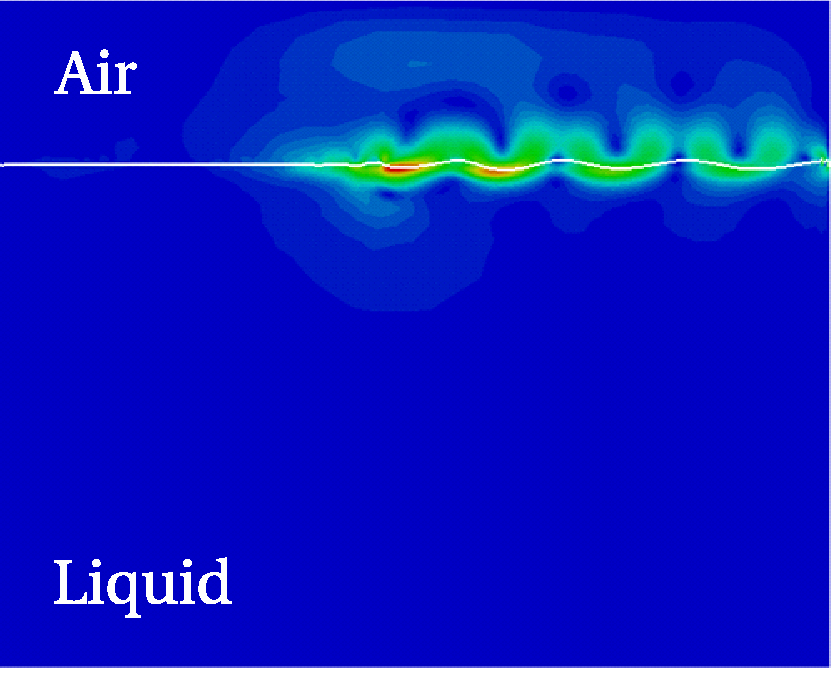
\includegraphics[width=\textwidth]{Chapter4/Graphics/UnstableInterface1.pdf}
	\caption{At a certain time increment (without mesh)}
    \label{fig:UnstableInterface1}
  \end{subfigure}
\qquad
 \begin{subfigure}[t]{0.4\textwidth}
    \centering
	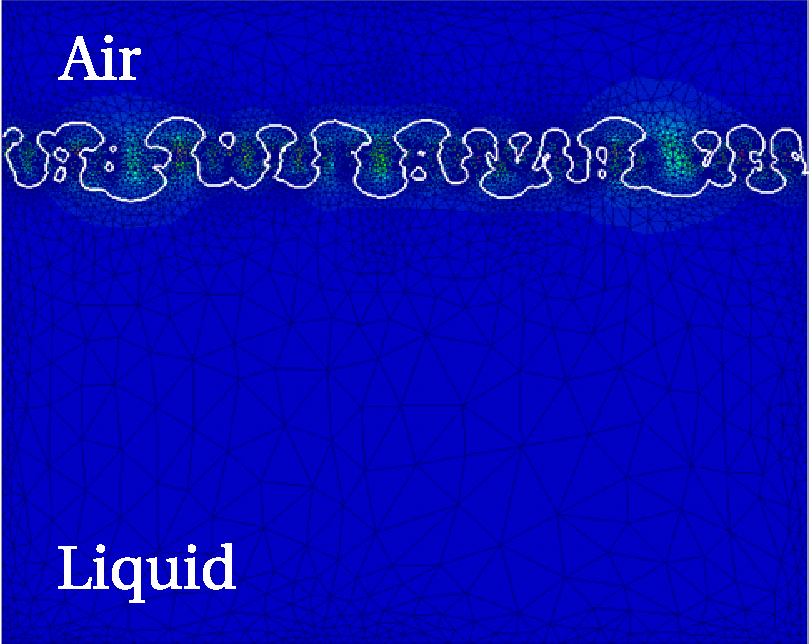
\includegraphics[width=\textwidth]{Chapter4/Graphics/UnstableInterface2.pdf}
	\caption{Another time increment (with mesh)}
    \label{fig:UnstableInterface2}
  \end{subfigure}
\caption{Interface destabilisation under the effect of high properties ratio across the interface.}
\end{figure}
%----------------------
%%---------

\subsubsection{Modified coupling}
In contrast to a classic coupling, here we attempt to modify the velocity field before feeding to the transport solver.
The main motivation for considering this approach is the lack of stability that we observed whenever the mechanical
properties of the fluids were different by several orders of magnitude.
The algorithm should simultaneously fulfil these requirements: 
\begin{itemize}
\itemsep0em
\item support high ratios of fluids density with close viscosities by preserving an non-oscillating interface,
\item maintain a horizontal level at the free surface of the melt,
\item follow shrinking metal surface profile in solidfying regions,
\item satisfy the mass conservation principle, essentially in the metal.
\end{itemize}
We want to process the original transport velocity by imposing a uniform motion (speed and direction) 
at the nodes of the free surface, and at the same time, be able to follow the pipe formation at the 
surface as a result of solidification shrinkage, as shown in \cref{fig:horizontal_liquid_surface}.

%----------------------
\begin{figureth}
% textwidth 
{0.8}
%path 
{Chapter4/Graphics/FreeSurface.pdf}
% caption
{Snapshot of a solidifying ingot by a cooling flux from the side. The profile of the actual surface changes in solid and mushy regions
to adapt the new density while staying perfectly horizontal in the liquid phase.}
% label
\label{fig:horizontal_liquid_surface}
\end{figureth}
%-----------------------------------
%
\comment{How to transport level set using velocity from momentum conservation DIRECTLY or AVERAGED PER ELEMENTS, 
show examples of instability/stability when using false/nominal air properties \\ 
Validation of LS transport: perform test case simulation of buoyancy driven air droplet in water by 2005Nagrath that I also have seen 
in Shyamprasad's masters report). => I didnt notice: what time step $\delta t$ did they use ? }
%
%----------------------
\begin{figureth}
% textwidth 
{0.8}
%path 
{Chapter4/Graphics/AvgTransport/BottomSideCooling.pdf}
% caption
{Treatment of liquid free surface in a) bottom and b) side heat extraction configurations. The dashed line represents the 
initial level of the free liquid surface.}
% label
\label{fig:bottom_side_cooling}
\end{figureth}
%-----------------------------------

The general idea is read the velocity around the interface up to a certain thickness, which may be the same 
thickness as the diffuse interface defined in \cref{sec:heaviside}, then compute a volumetric average
from all the elements in the thickness. This average is then given to the transport solver, which will apply
the same magnitude and direction to transport the interface. However, as we only need the transport velocity
to be uniform within the "100\% liquid" elements, it should not be the case for the other elements that belong 
either to the mushy zone or the solid region, where shrinkage is taking place.
Therefore, depending on the heat extraction configuration, two scenarios are possible. If heat extraction is far from
the interface, i.e. there is not direct contact as in \cref{fig:bottom_side_cooling}a, 
the surface area remains unchanged at any time, hence all the elements
around the interface are "100\% liquid". This happens when a bottom cooling is applied to the ingot. In contrast, if a side cooling 
is applied as shown in \cref{fig:bottom_side_cooling}b, the surface area of the interface will be reduced over time
as a consequence of the solid front progression. In this case, the average transport velocity should be computed only
from the elements belonging to the free surface. The remaining part of the interface which belongs to partial or full 
solid regions, is transported with Navier-Stokes output, which should be some orders of magnitude less than the velocity
imposed at the free surface, as a result of a decreasing permeability.

%
%--------------------------------
%--
\section{1D application: \bin{Al}{7}{Si}}
%--------------------------------------------
\subsection{Geometry and boundary conditions}
A simple but very efficient way of analysing the model is to test it through a 1D flow configuration with energy and species conservation.
For this purpose, we take an aluminium-silicon alloy with the same properties used for the thermal solver validation in \cref{table:data_case_alsi7}.
The major difference with respect to the former validation setup is the air domain that should also be included in the mesh.
We consider a 2D rod having as dimensions \SI{0.14}{\metre}$\times$\SI{0.001}{m}, where initially the air column's height is only \SI{0.04}{\metre}
and the remainder of the length is for the metal.  
\textbf{FIGURE} shows the geometry, mesh used for this section simulations, while \textbf{FIGURE} shows the thermal and mechanical boundary conditions.
In the latter, velocity-slip conditions were imposed on the lateral boundaries while a no-slip was used at the bottom where heat is extracted,
to ensure a 1D air flow from the free air inlet at the top. 

In this case, imposing slip conditions on lateral sides is two-fold: on one hand, we need to ensure that the fluid flow solution
remain one-dimensional, hence symmetry on the boundaries solves the issue, while on the other hand during solidification, 
the resulting feeding flow should be able to transport the interface intersecting with boundary nodes. If boundary velocities
are zero, then the interface transport will face problems at these boundary nodes. This is indeed an important and relevant point 
in the next 2D test case.

%
%-----------------
\begin{figure}[htbp]
\centering
   %------------
  \begin{subfigure}[t]{0.45\textwidth}
    \centering
	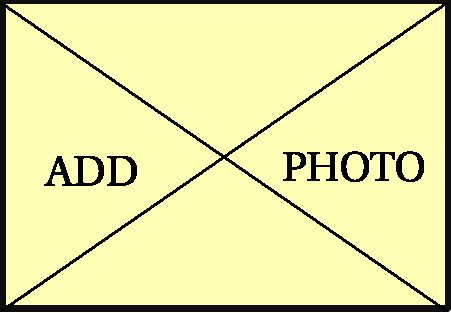
\includegraphics[width=\textwidth]{Misc/dummy.pdf}
	\caption{}
    \label{fig:1d_alsi7_geo}
  \end{subfigure}
   %------------
   \begin{subfigure}[t]{0.45\textwidth}
    \centering
	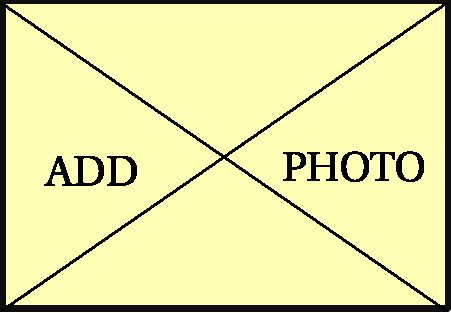
\includegraphics[width=\textwidth]{Misc/dummy.pdf}
	\caption{}
    \label{fig:1d_alsi7_bc}
  \end{subfigure}
  %-------- 
\caption{Geo and boundary conditions} 
\label{fig:}
\end{figure}
%-----------------
%
\subsection{Shrinkage without macrosegregation}
%----------------------------------------------------

The first simulation is the solidification without any segregation, hence a unique solidification path is considered at $\Cnominal=$\bin{Al}{7}{Si},
shown in \cref{fig:shrinkage_nomacro_sp}.
This case is interesting as a reference case, where we can study volume shrinkage and level set behaviour in a simple segregation-free configuration.
We first use a homogeneous isotropic mesh of constant size $h=$ \SI{200}{\micro \metre}. The liquid and solid phase densities are assumed constant
and respectively equal to \SI{2600}{\udensity} and \SI{2800}{\udensity}. This density difference is equivalent to a ratio of $\beta_{SS}= \brac{\rhos-\rhol}/\rhos$,
also termed as \emph{solidification shrinkage} by \citet{flemings_macrosegregation:_1967}. 
In the current conditions, $\beta_{SS}$ is constant and equal to \SI{7.14}{\percent}. 
The domain is initially meshed before any resolution, as shown in \cref{fig:1dalsi7_lsmixing}, in a way to reduce interpolation errors that may
cause coarse elements within the transition of fluids density and dynamic viscosity, reminding that these parameters are crucial for the stability 
of the velocity solution used later in the transport step. The chosen mixing laws are arithmetic for the density and logarithmic for the viscosity.
The choice is based on tests done in former Ph.D. projects at CEMEF. The initial mesh sizes are given in \cref{table:1dalsi7_meshsize}.

%--------------------------------
\begin{table}[htbp]
\centering
\caption{Summary of the different mesh sizes used to generate an adaptive anisotropic mesh, along with the level mixing thickness, $\varepsilon$. 
Refer to \cref{sec:remesh2_params} for the definition of each mesh parameter.}
\label{table:1dalsi7_meshsize}
{\tabulinesep=1.0mm \begin{tabu}{ll}
\tabucline[1pt]{-}
\textbf{Mesh parameter} & \textbf{Size [\si{\metre}]} \\\tabucline[1pt]{-}
%-----------------------------
$\varepsilon $			&	\num{2.5e-4}	\\
$h_{\vec{n}}$ 			&	\num{2.5e-5}	\\ 
$h_{\vec{\tau}}$ 		&	\num{2e-4}		\\ 
$h_M$  					&	\num{1.5e-4}	\\
$h_A$  					&	\num{2.5e-4} \\\tabucline[1pt]{-}
%-----------------------------
\end{tabu}}
\end{table}
%--------------------------------

%--------------
\begin{figureth}
% textwidth 
{1.0}
%path 
{Chapter4/Graphics/1d/ls_mixing.pdf}
% caption
{Snapshots of the initial adapted mesh around the interface with different mesh sizes in the air and the metal. The adapted region
is stretched beyond the level set mixing thickness to ensure better interpolation around the interface, in case of emergence of diffusion
instabilities. To the right, the reference fluid density and viscosity are plotted in the transition zone, showing a symmetric mixing for the former
and a shifted mixing for the latter, as a consequence of the mixing laws.
The thick blue line represents the zero iso-value of the distance function.}
% label
\label{fig:1dalsi7_lsmixing}
\end{figureth}
%--------------

%--------------------------------------
\begin{figure}[htbp]
\centering
\begin{tikzpicture}
 \pgfkeys{%
    /pgf/number format/set thousands separator = {}}
\begin{axis}
[
	table/col sep=comma,
	smooth, %ybar
	%stack plots=y,
	%area style,
	enlarge x limits=false,
	legend pos=north west,
	scaled ticks=true,
	xlabel=Temperature (\si{\udegC}),
	ylabel=Volume fraction (-),
	xticklabel style={/pgf/number format/fixed},
	xtick={577, 600, 618},
	%x tick label style={rotate=45,anchor=east},
	%width=0.5\textwidth,
	mark repeat	= {2},
]
\addplot table [x=Temperature, y expr=\thisrow{LIQ}] {Chapter4/Data/1d_alsi7_nominalSP/sp.csv} \closedcycle ;
\addplot table [x=Temperature, y expr=\thisrow{ALPHA}] {Chapter4/Data/1d_alsi7_nominalSP/sp.csv}\closedcycle;
\addplot table [x=Temperature, y expr=\thisrow{BETA}] {Chapter4/Data/1d_alsi7_nominalSP/sp.csv}\closedcycle;

\legend{Liquid, BCC, FCC}
\end{axis}
\end{tikzpicture}

\caption{Unique solidification path at nominal composition for the shrinkage case without macrosegregation.}
\label{fig:shrinkage_nomacro_sp}
\end{figure}
%--------------------------------------

At a first glance, results show that the interface stability is compromised by a chosen time step for a given mesh size, and that the interface dynamics
require attention even before investigating the feeding flow created by solidification. As a demonstration, \cref{fig:1dalsi7_velocity_dt} shows different
time steps with the same adaptive meshing parameters. For time steps greater than 0.01 s, Navier-Stokes computations did not converge resulting in an high artificial 
flow quickly destabilising the interface. It should be noted that the frame corresponding to 0.02 s was taken at an earlier time than the two other frames.

%--------------
\begin{figureth}
% textwidth 
{0.6}
%path 
{Chapter4/Graphics/1d/ls_velocity_dt.pdf}
% caption
{Three average fluid velocity frames at different time steps: 0.005 s, 0.01 s and 0.02 s. The first and second frame are taken after 
50 seconds of cooling while for the last frame, the frame was taken after only 1 second of cooling, thus it is crossed to show non-convergence.
The thick black line represents the zero iso-value of the distance function.}
% label
\label{fig:1dalsi7_velocity_dt}
\end{figureth}
%--------------

Although no solidification has yet started at 100 s, a two-dimensional flow is observed around the interface, while tends to \SI{e-8}{\uvelocity} elsewhere in the ingot.
\Cref{fig:1dalsi7_velocity_dt} confirms that this flow is still predicted at smaller time steps. This flow seems like a pure numerical response
to the properties jump across the interface, namely density and dynamic viscosity. It is also noted that the interface position
is not modified by the neighbouring currents, that reach a maximum magnitude of \SI{e-4}{\uvelocity}. Therefore, the optimal time step 
for this simulation is set to 0.01 s, and we refer to it as case R, which stands for "real" air.

The fact that properties transition is crucial in the solution stability, is investigated by 2 reference cases, having equal properties 
(density and dynamic viscosity) but with different time steps, 0.01 (case A1) and 0.1 s (case A2), where "A" stands for artificial.
All simulation cases are grouped in \cref{table:1dalsi7_comparative_nomacro}.

%--------------------------------
\begin{table}[htbp]
\centering
\caption{Summary of the comparative shrinkage simulations without macrosegregation.}
\label{table:1dalsi7_comparative_nomacro}
{\tabulinesep=1.0mm \begin{tabu}{llll}
\tabucline[1pt]{-}
\textbf{Case} & \textbf{Air viscosity [\si{\uviscosity}]} & \textbf{Air density [\si{\udensity}]} & \textbf{Time step [s]} \\\tabucline[1pt]{-}
%-----------------------------
A1			& \num{e-3}	&	\num{2600}	&	0.01		\\
A2			& \num{e-3}	&	\num{2600}	&	0.1	\\
R			& \num{e-4}	&	\num{1.3}	&	0.01	\\\tabucline[1pt]{-}
%-----------------------------
\end{tabu}}
\end{table}
%--------------------------------

When the air subdomain is given the metal's properties, it becomes denser and more viscous by several orders of magnitude. 
\Cref{fig:1dalsi7_caseA1A2}, in which cases A1 and A2 are compared, shows no noticeable sign of velocity instability near the interface before 200 s.
It can be explained by the fact that the air behaves mechanically like a fluid metal given similar properties, 
therefore no steep transitions are computed at the interface. 
However, it is interesting to compare results of \cref{fig:1dalsi7_equalprops_smallstep1} and \cref{fig:1dalsi7_equalprops} at 600 s.
For case A1, the interfaces is slightly skewed due to slower flow at the left side of the interface, while for case A2, the flow disturbs
the interface deforming it until the end of solidification, as seen at 1000 s. This shows the importance of the chosen time step
in both the Navier-Stokes solver. 
We can also notice a common issue for all three case, A1, A2 and R, approximately at 400 s, the mushy zone enters within the diffuse interface, 
affecting the level set transport and thus causing mass conservation problems. These problems are discussed in the next section.

In contrast, \cref{fig:1dalsi7_differentprops} shows more viable results as far as the level set transport is concerned.
From 200 s to 800 s, the local flow instability (discussed earlier in \cref{fig:1dalsi7_velocity_dt}) is sustained, even until after solidification is complete.
However, in regions of 100\% metal and 100\% air the computed velocity is nearly the same order of magnitude as predicted for all three simulations.
Finally, in \cref{fig:1dalsi7_differentprops}, we notice a recirculating air flow in the vicinity of the interface as no metal shrinkage 
may further occur once solidification is complete, thus air flows freely in and out 
of the upper boundary with a very low magnitude ($\sim$ \SI{e-7}{\uvelocity}), while impinging on the air-metal surface.
Regarding the CPU times, cases A1 ran for 14 hours, case A2 took only 2 hours while case R ran for 23.3 hours.
%-----------------------------------------
\begin{figure}[htbp]
\centering
%======
  \begin{subfigure}{0.6\textwidth}
  \centering
    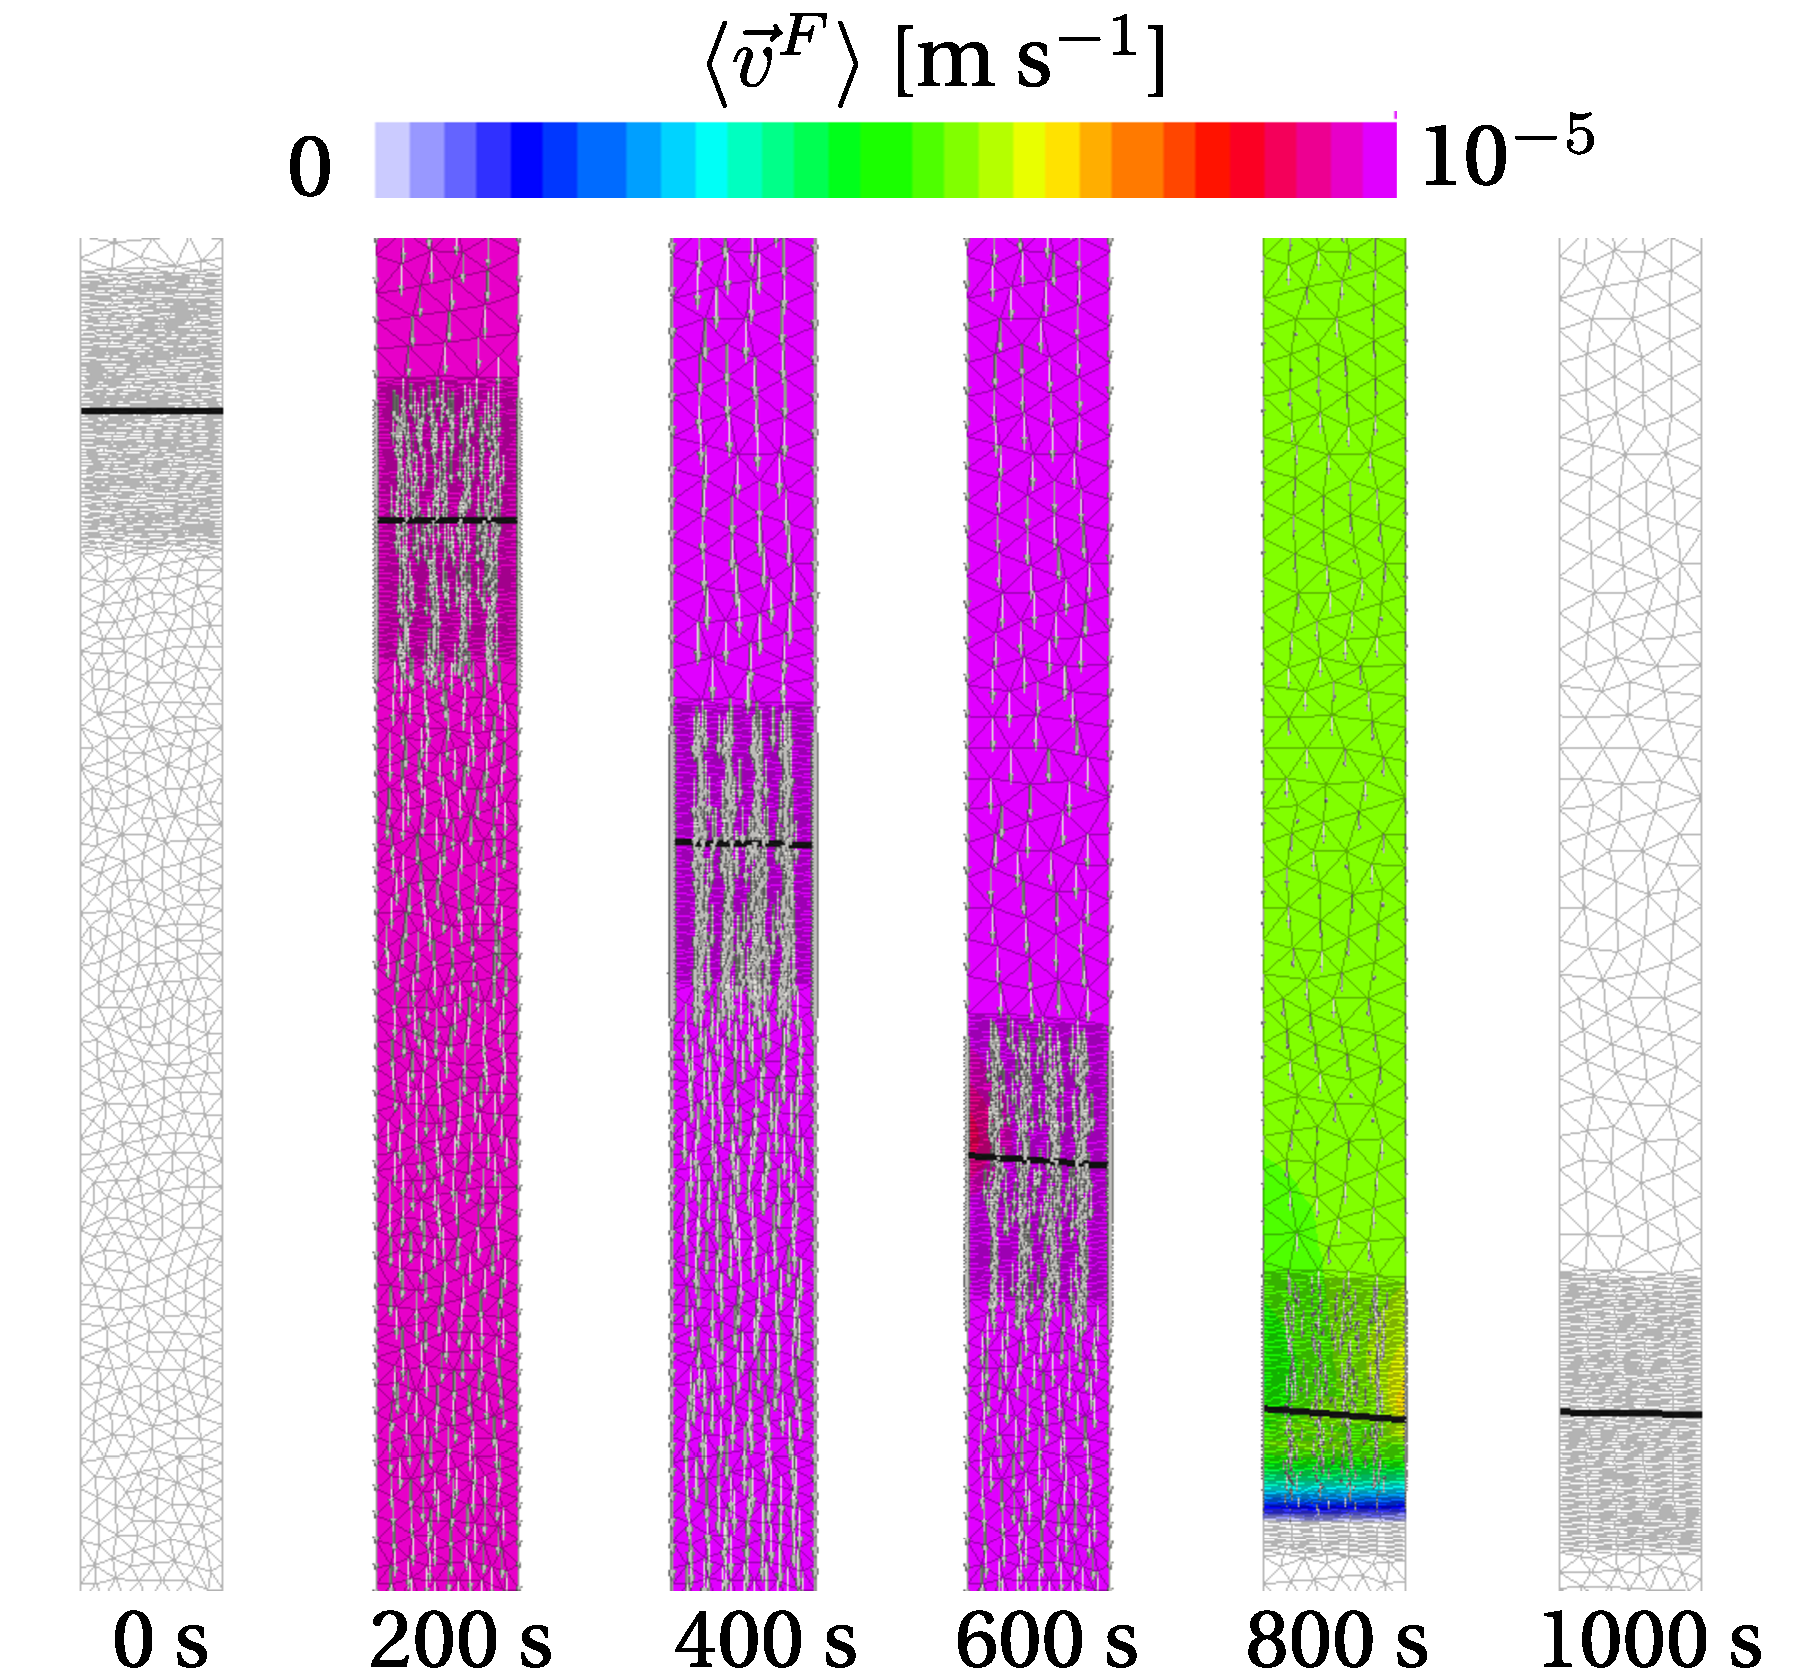
\includegraphics[width=\textwidth]{Chapter4/Graphics/1d/ls_velocity_equalprops_1e-2.pdf}
	\caption{Case A1}
    \label{fig:1dalsi7_equalprops_smallstep1}
  \end{subfigure}  
%======
\vskip\baselineskip
%======
  \begin{subfigure}{0.6\textwidth}
    \centering
    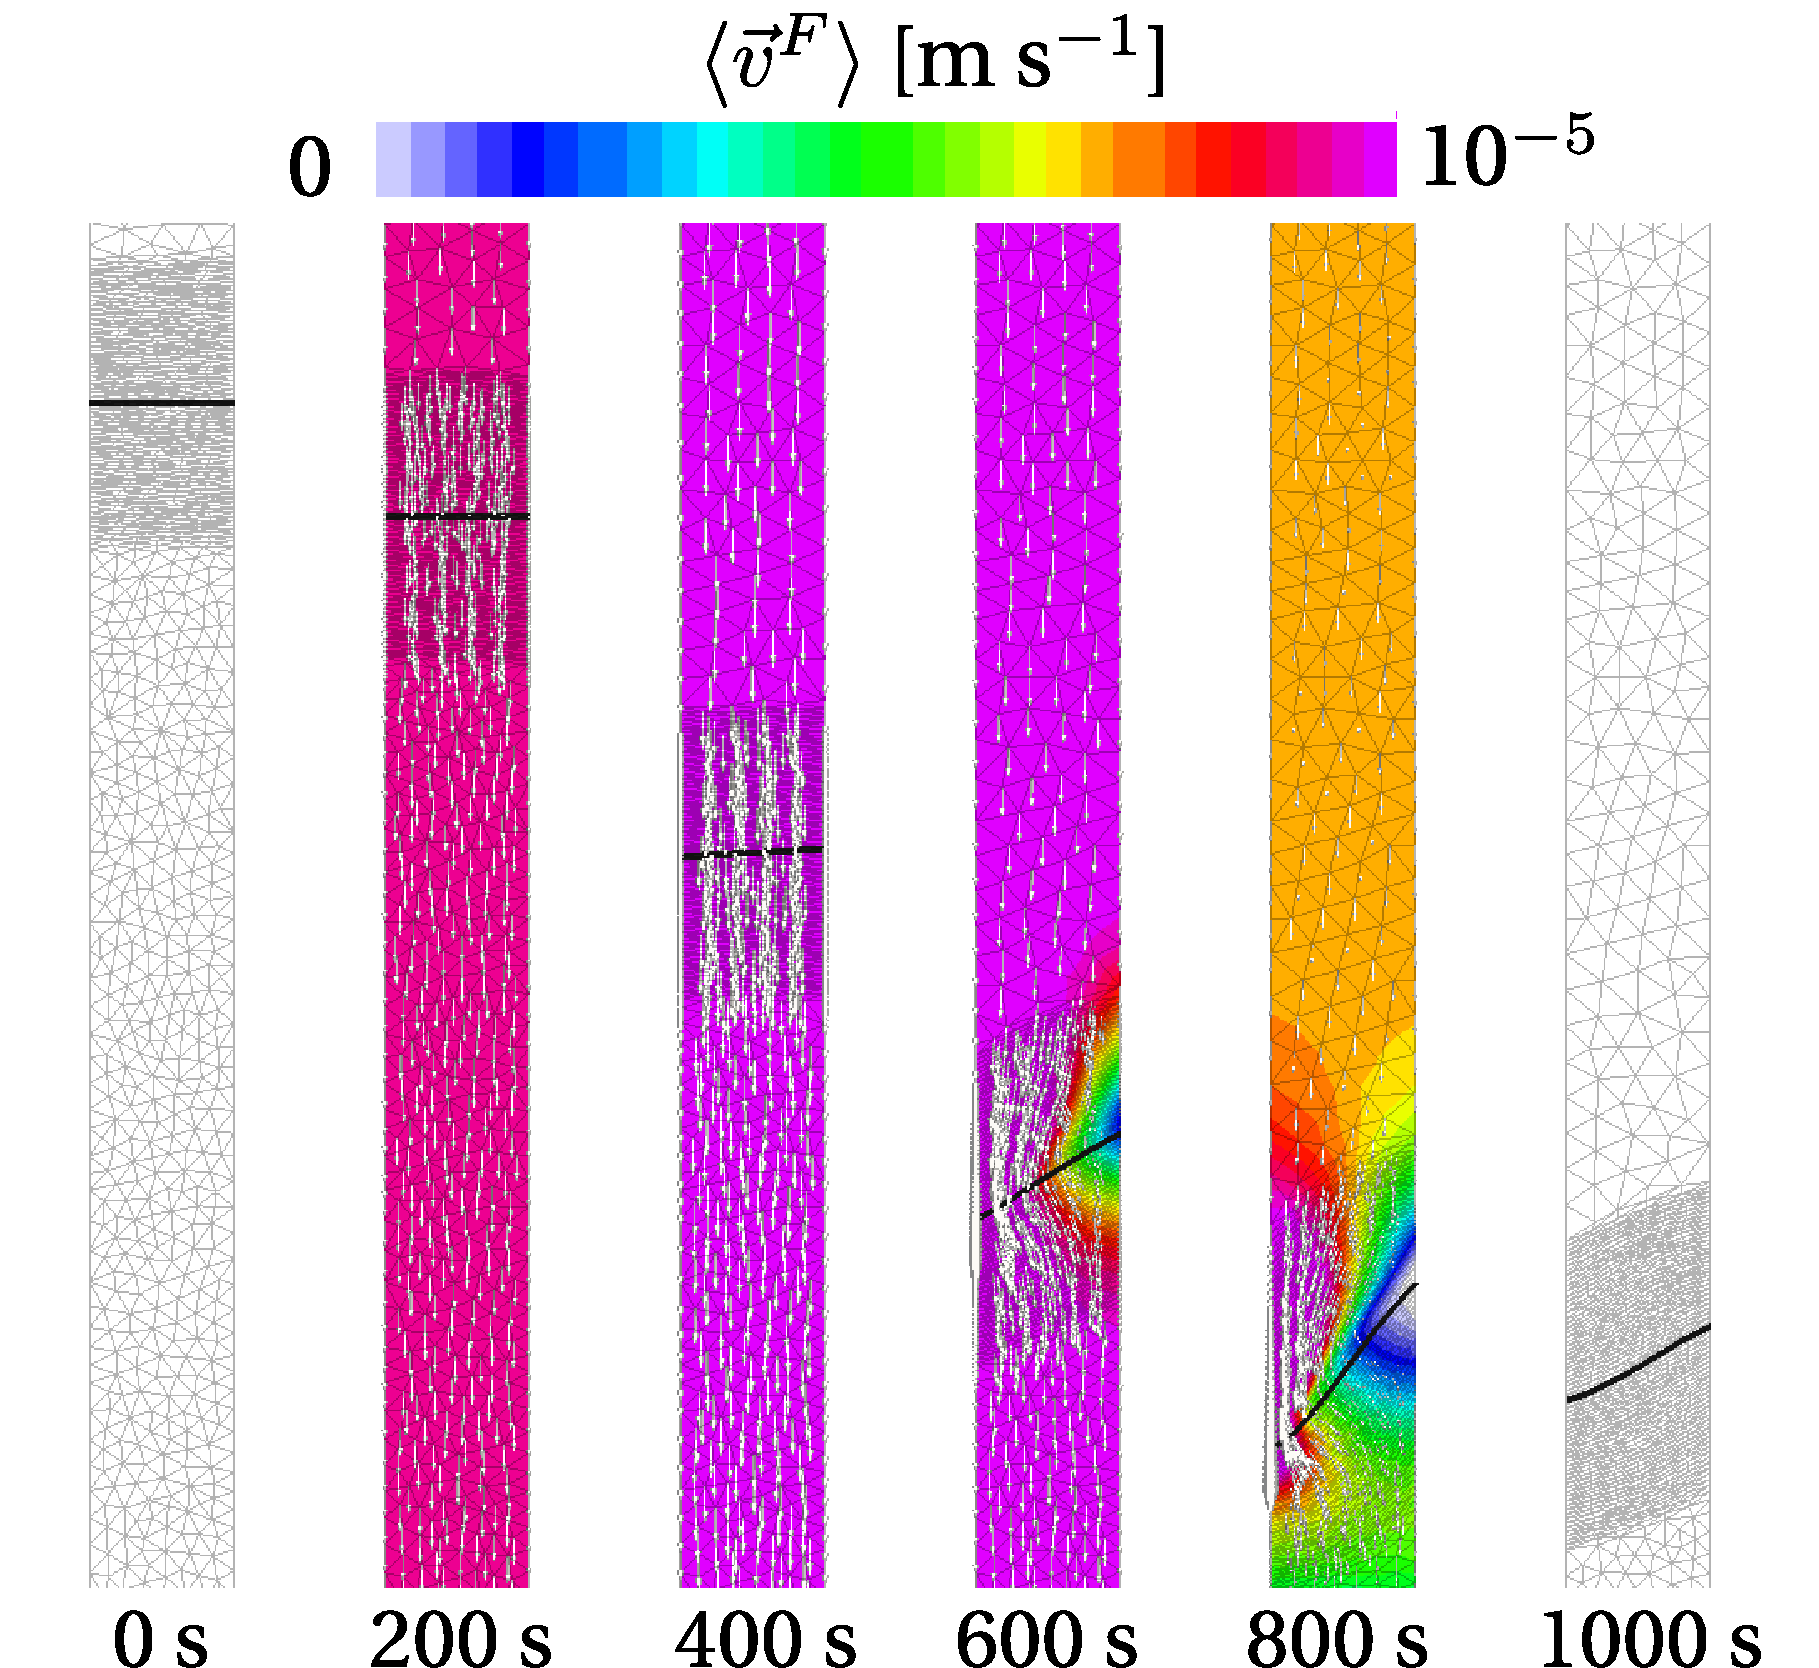
\includegraphics[width=\textwidth]{Chapter4/Graphics/1d/ls_velocity_equalprops.pdf}
	\caption{Case A2}
    \label{fig:1dalsi7_equalprops}
  \end{subfigure}
%======
\caption{Comparison of two simulations in several stages of solidification ending shortly after 800 s.
The results shows the influence of density and viscosity properties across the level set interface.
The plotted field is the average fluid velocity, on which the corresponding nodal vectors are superimposed, pointing
towards the solidification front. The thick black line represents the zero iso-value of the distance function.}
\label{fig:1dalsi7_caseA1A2}
\end{figure}
%-----------------------------------------

%-----------------------------------------
\begin{figure}[htbp]
\centering
%======
  \begin{subfigure}{0.6\textwidth}
  \centering
    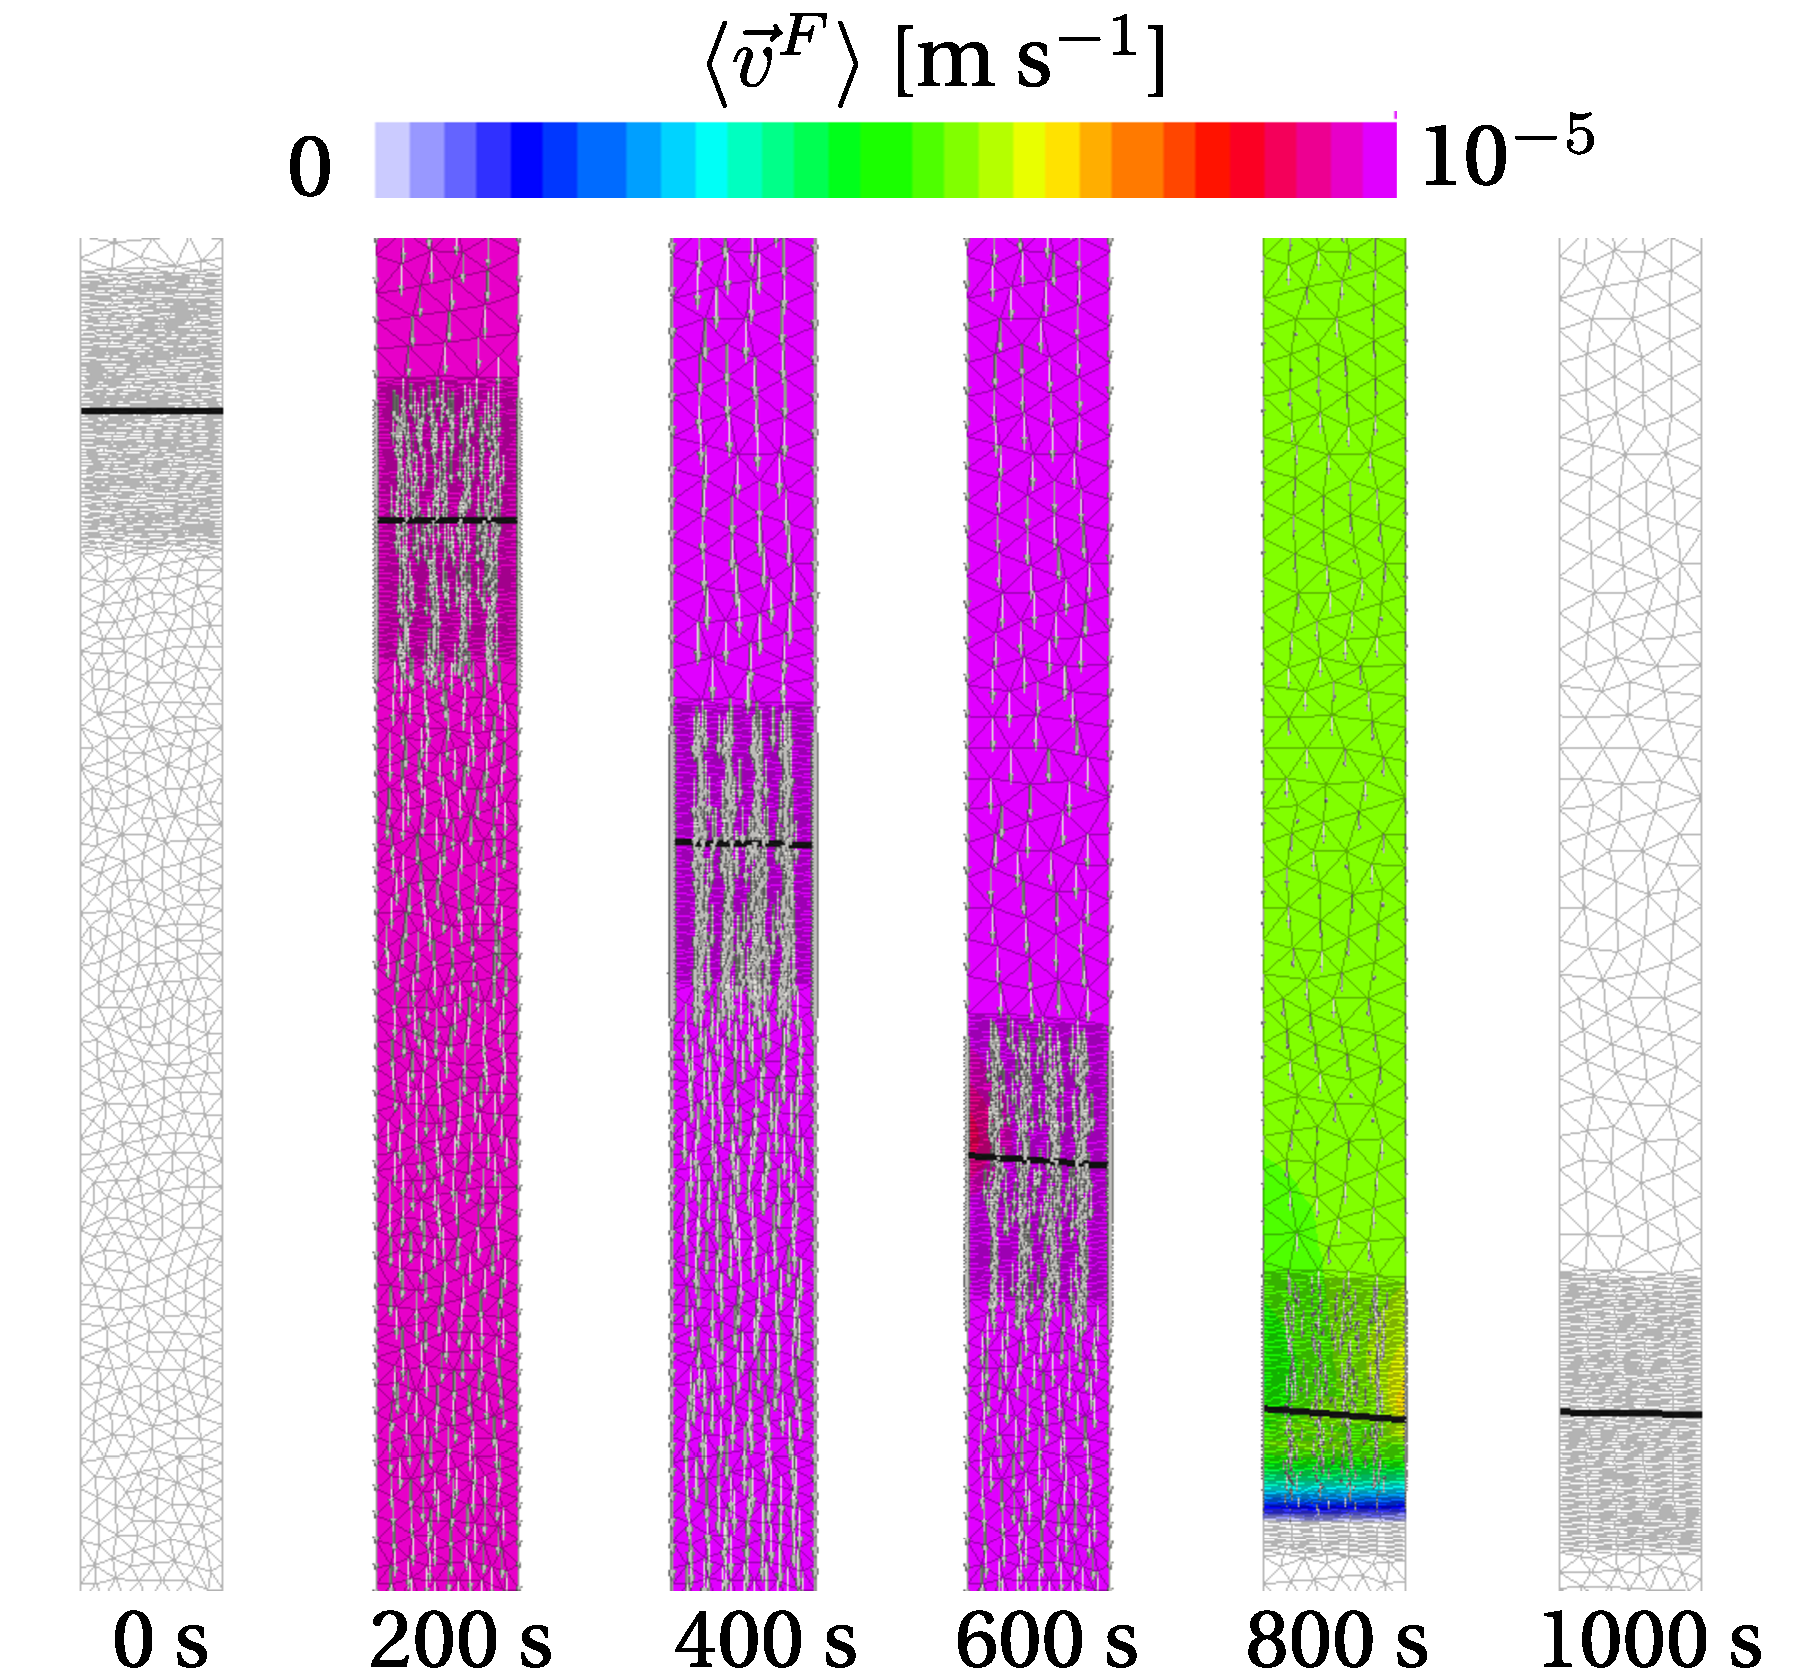
\includegraphics[width=\textwidth]{Chapter4/Graphics/1d/ls_velocity_equalprops_1e-2.pdf}
	\caption{Case A1}
    \label{fig:1dalsi7_equalprops_smallstep2}
  \end{subfigure}  
%======
\vskip\baselineskip
%======
  \begin{subfigure}{0.6\textwidth}
    \centering
    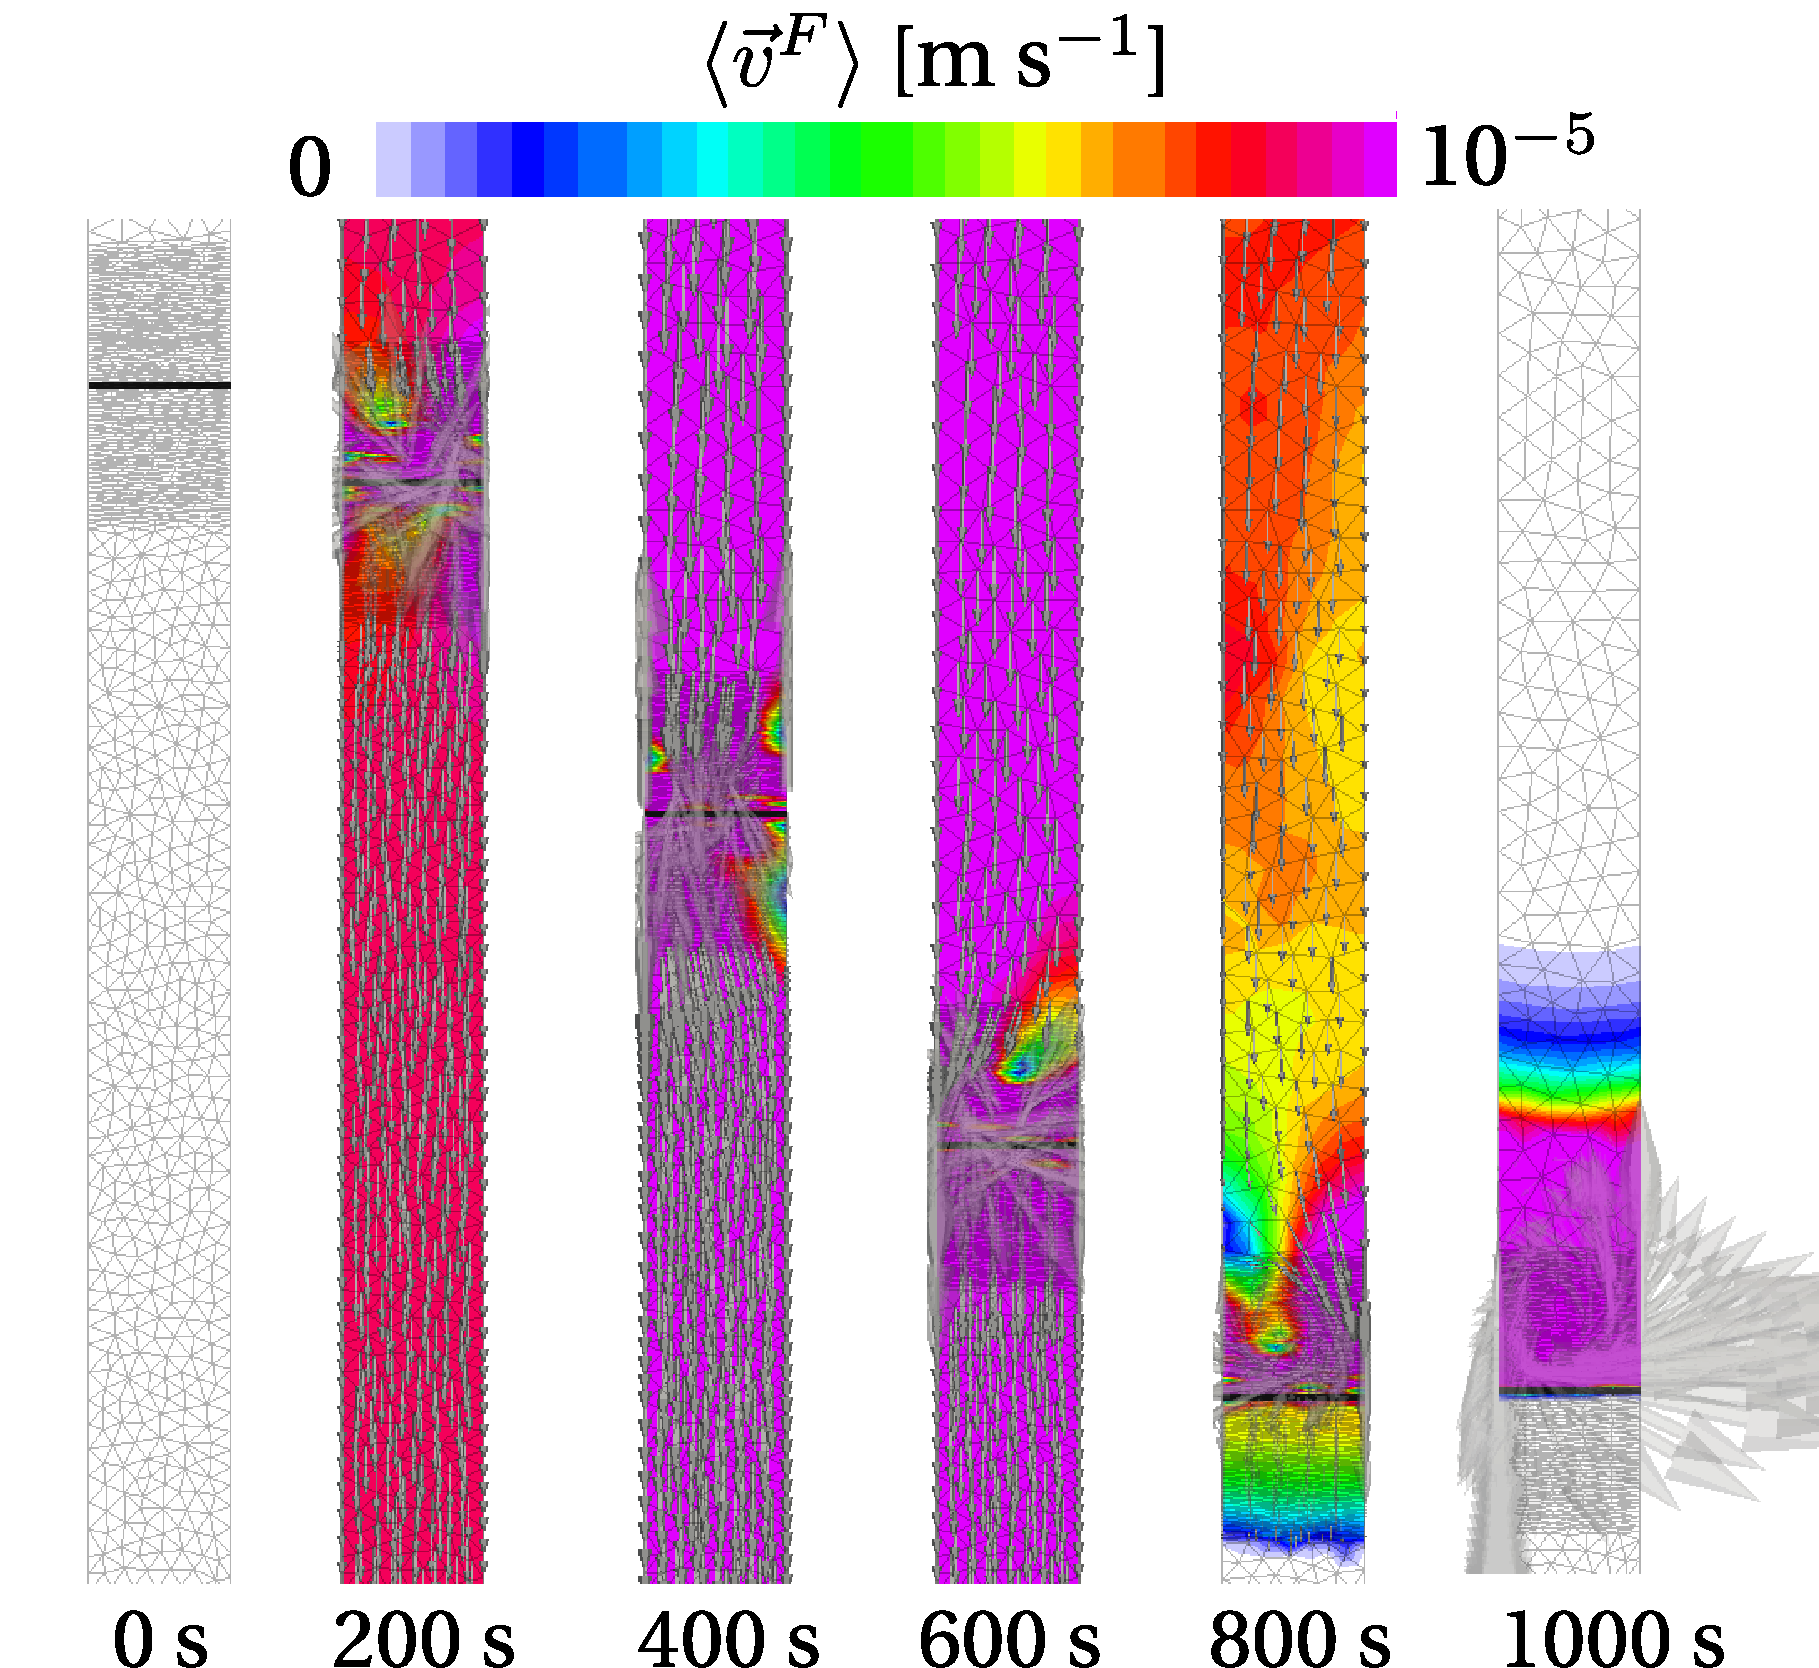
\includegraphics[width=\textwidth]{Chapter4/Graphics/1d/ls_velocity_differentprops.pdf}
	\caption{Case R}
    \label{fig:1dalsi7_differentprops}
  \end{subfigure}
%======
\caption{Comparison of two simulations in several stages of solidification ending shortly after 800 s.
The results shows the influence of density and viscosity properties across the level set interface.
The plotted field is the average fluid velocity, on which the corresponding nodal vectors are superimposed, pointing
towards the solidification front. The thick black line represents the zero iso-value of the distance function.
The vectors were made transparent in the transition zone so as not to hide the interface level.}
\label{fig:1dalsi7_caseA1R}
\end{figure}
%-----------------------------------------

\subsubsection{Mass conservation study}

The previous computations showed that the mass conservation, which is the consequence of the level set transport,
can be lost. In order to better understand the process, we define the metal's mass as a function of the 
metal's average density and the Heaviside function relative to the metal subdomain, as follows:
%----------------
\begin{align}
\label{eq:metal_mass}
& m^M = \integral{\Ohm}{H^M \avg{\rho}^M}{\Ohm}	
\end{align}
%---------------
Then, the mass conservation can be monitored by processing \cref{eq:metal_mass} at each time step, and computing
the relative mass change by writing:
%----------------
\begin{align}
\label{eq:metal_mass_variation}
&  m^M_\% = \frac{m^M - m^M_i}{m^M_i} \times 100	
\end{align}
%---------------
The relative mass change gives us information on the level set transport.
As the current case is 1D and phase densities are constant throughout the simulation, mass conservation can be 
checked by a much simpler than by checking \cref{eq:metal_mass_variation}. Since we know the initial metal's column
length, $l^M_0$, and the expected solidification shrinkage is \SI{7.14}{\percent}, we should expect a final length of 
$l^M_f= \brac{1-\beta_{SS}} l^M_0 =$  0.09286 \si{\metre}. However, this equation is very useful and applicable in 2D and 3D
cases of solidification shrinkage.
%--------------------------------------
\begin{figure}[htbp]
\centering
\begin{tikzpicture}
 \pgfkeys{%
    /pgf/number format/set thousands separator = {}}
%================================================
\begin{axis}
[	name=artificial,
	title=(a) Case A1,
	scale only axis,
	table/col sep=tab,
	enlarge x limits=false,
	legend pos=north west,
	scaled ticks=true,
	xlabel=Time (s),
	ylabel=$m^M_\%$ (\%),
	xticklabel style={/pgf/number format/fixed},
	xtick={0,200,400,600,800,1000},
	ytick={-0.1,0,0.1,0.2},
	%x tick label style={rotate=45,anchor=east},
	width=0.4\textwidth,
	%height=5cm,	
	ymin=-0.1, ymax=0.2,
	mark repeat	= {30},
]
\addplot table [x=Temps, y=mMpct] {Chapter4/Data/1d_alsi7_mass/ArtificialDarcyBlocking0pct_smallstep.txt} \closedcycle ;
%\addplot table [x=Temps, y=mMpct] {Chapter4/Data/1d_alsi7_mass/ArtificialDarcyBlocking25pct.txt}\closedcycle;
%\addplot table [x=Temps, y=mMpct] {Chapter4/Data/1d_alsi7_mass/ArtificialDarcyBlocking50pct.txt}\closedcycle;
%\addplot table [x=Temps, y=mMpct] {Chapter4/Data/1d_alsi7_mass/ArtificialDarcyBlocking99pct.txt}\closedcycle;
%\legend{Blocking at 0\% $\gl$, Blocking at 25\% $\gl$, Blocking at 50\% $\gl$, Blocking at 99\% $\gl$}
\end{axis}
%================================================
%\hfill
%================================================
\begin{axis}
[	name=real,
	title=(b) Case R,
	at=(artificial.right of south east), anchor=left of south west,
	scale only axis,
	%yticklabel pos=left,
	table/col sep=tab,
	enlarge x limits=false,
	legend pos=north west,
	scaled ticks=true,
	xlabel=Time (s),
	xticklabel style={/pgf/number format/fixed},
	xtick={0,200,400,600,800,1000},
	ytick={-0.1,0,0.1,0.2},
	yticklabels={},
	%x tick label style={rotate=45,anchor=east},
	width=0.4\textwidth,
	%height=5cm,	
	ymin=-0.1, ymax=0.2,
	mark repeat	= {30},
]
\addplot table [x=Temps, y=mMpct] {Chapter4/Data/1d_alsi7_mass/RealDarcyBlocking0pct.txt} \closedcycle ;
%\addplot table [x=Temps, y=mMpct] {Chapter4/Data/1d_alsi7_mass/RealDarcyBlocking25pct.txt}\closedcycle;
%\addplot table [x=Temps, y=mMpct] {Chapter4/Data/1d_alsi7_mass/RealDarcyBlocking50pct.txt}\closedcycle;
%\addplot table [x=Temps, y=mMpct] {Chapter4/Data/1d_alsi7_mass/RealDarcyBlocking99pct.txt}\closedcycle;
%\legend{Blocking at 0\% $\gl$, Blocking at 25\% $\gl$, Blocking at 50\% $\gl$, Blocking at 99\% $\gl$}
\end{axis}
\end{tikzpicture}
%================================================
\caption{Variation of the metal's mass versus solidification time in cases A1 and R.}
\label{fig:shrinkage_nomacro_massconserv}
\end{figure}
%--------------------------------------

%cases: from 0\%, i.e. where the transport velocity is given by the Navier-Stokes-Darcy resolution, up to 99\% which means that once a node's liquid fraction becomes less than 99\%, 
%its transport velocity becomes zero. Note that the blue curve corresponds to the results shown in \cref{fig:1dalsi7_equalprops}.

In the previous section, we observed transport problems taking place around 400 s of cooling. Although it was clearly seen in \cref{fig:1dalsi7_equalprops}, it applies
for both cases, whether air properties are equal or different than the liquid's properties across the interface. 
The mass variation plots in \cref{fig:shrinkage_nomacro_massconserv} confirm these observations.
Therefore, we can deduce that regardless of the time step and the level set mixing of properties, 
transport problems may occur. 

The level set method is known to have poor mass conservation properties. However, the mass variation
we see in the previous plots is more related to a physical problem: \textbf{at which velocity does the interface move?}
In our simulations, we systemically considered the Navier-Stokes solution $\vitf$,
to transport the metal-air interface. This solution is equal to $\vit= \gl \vl$ in the metal subdomain. 
However in reality, 
between the metal and the air, two interfaces exist: the liquid-air ($\liqair$) and solid-air ($\solair$) interfaces, and these interfaces move at different velocities as solidification proceeds.
The liquid-air interface exists at early stages of solidification where only liquid is in contact with the air. In later stages,
the mushy zone delimited by dendrite tips, reaches the free liquid surface, creating hence these distinct interfaces: a first interface separating
interdendritic liquid from the air, and a second interface that separates the dendrites also from the air. The $\liqair$ interface is driven
by solidification shrinkage and therefore by the real microscopic velocity of the interdendritic liquid, $\vl$. According to \citet{dantzig_solidification_2009},
this velocity is constant when the solidification shrinkage and the isotherms velocity $\vec{v}_T$ are constant, as states the equation:
%----------------
\begin{align}
\label{eq:real_velocity}
& \vl = -\beta_{SS} \vec{v}_T
\end{align}
%---------------
As for the $\solair$ interface, its motion is induced by a mechanical deformation of the solid phase either due to thermal shrinkage or external mechanical stresses.
The first factor is ubiquitous in any solidification process, while the second factor is process-dependent. 
In the present work, we remind that the solid phase is assumed fixed and rigid, therefore we consider dendrites
to be undeformable during their growth. Unfortunately, this assumption is contradictory with our current situation where the metal keeps shrinking, 
until an overlap between the level set's diffuse interface and and the mushy zone overlap, as shown in \cref{fig:1dalsi7_interface_stages}).
At this stage, tracking a single interface induces concept errors, because we are not sure which of the previously mentioned interfaces is being tracked, and hence failing
to determine an adequate transport velocity field. 

\begin{figureth}
% textwidth 
{0.8}
%path 
{Chapter4/Graphics/1d/interface_stages.pdf}
% caption
{Schematic describing the physical (first row) and numerical (second row) process of moving an interface between air and metal subdomains, in three intermediate stages of 
solidification.}
% label
\label{fig:1dalsi7_interface_stages}
\end{figureth}
%--------------


In the light of these facts, we will try to limit as much as possible the interface motion, once the mushy zone has reached the diffuse interface.
To do so, we firstly advise to keep a very small thickness interface, in order to delay the previously explained overlap. Moreover, we suggest computing the 
transport velocity, used in \cref{eq:transport_weak1}, at each node $j$ as follows:
%--------
\begin{align}
\label{eq:}
\vec{v} =
\begin{cases}
  \vit_j 	& \text{ if } g^l_j > g^{BL} \\
  0 		& \text{otherwise}
\end{cases}
\end{align}
%---------------
where $g^{BL}$ is the threshold for the liquid fraction, below which we consider that the interface should not be transported.
\Cref{fig:massconserv_blockingpct} shows the mass variation for three blocking fractions: 0, 50, 75 and 99 percent.
The first value corresponds the case where the Navier-Stokes solution is directly passed to the transport solver.
For the last value, the portion of the interface in contact with the low solid fraction part
of the mushy zone becomes immobile. It is clearly seen that the consequence on the mass conservation is not very good, as 
the mass increases up to 3\% while the eutectic front is consuming the liquid within the mushy zone, while no further shrinkage is allowed.

%--------------------------------------
\begin{figure}[htbp]
\centering
\begin{tikzpicture}%[spy using outlines={draw, blue, magnification=2, connect spies}]
 \pgfkeys{%
    /pgf/number format/set thousands separator = {}}
%================================================
\begin{axis}
[	name=mass curves,
	%title= mass conservation,
	scale only axis,
	table/col sep=tab,
	enlarge x limits=false,
	legend pos=north west,
	scaled ticks=true,
	xlabel=Time (s),
	ylabel=$m^M_\%$ (\%),
	xticklabel style={/pgf/number format/fixed},
	xtick={0,200,400,600,800,1000},
	%ytick={-0.1,0,0.1,0.2},
	%x tick label style={rotate=45,anchor=east},
	width=0.5\textwidth,
	%height=5cm,	
	%ymin=-0.1, ymax=0.2,
	mark repeat	= {30},
]
%\coordinate (pt) at (axis cs:500,0);
%\coordinate (posZoom) at (axis cs:100,0.5);
\addplot table [x=Temps, y=mMpct] {Chapter4/Data/1d_alsi7_mass/RealDarcyBlocking0pct.txt} \closedcycle ;
\addplot table [x=Temps, y=mMpct] {Chapter4/Data/1d_alsi7_mass/RealDarcyBlocking50pct.txt} \closedcycle ;
\addplot table [x=Temps, y=mMpct] {Chapter4/Data/1d_alsi7_mass/RealDarcyBlocking75pct.txt} \closedcycle ;
\addplot table [x=Temps, y=mMpct] {Chapter4/Data/1d_alsi7_mass/RealDarcyBlocking99pct.txt} \closedcycle ;
\legend{$g^{BL}=0\%$, $g^{BL}=50\%$, $g^{BL}=75\%$, $g^{BL}=99\%$}
%----
%\begin{scope}
%	\spy on (pt) in node at (posZoom);
%\end{scope}
\end{axis}
\end{tikzpicture}
\caption{Relative mass change versus time for different blocking fractions $g^{BL}$ in the transport solver.}
\label{fig:massconserv_blockingpct}
\end{figure}
%--------------------------------------
%================================================

\begin{figure}[htbp]
\centering
\begin{tikzpicture}%[spy using outlines={draw, blue, magnification=2, connect spies}]
 \pgfkeys{%
    /pgf/number format/set thousands separator = {}}
%================================================
\begin{axis}
[	name=mass curves,
	%title= mass conservation,
	scale only axis,
	table/col sep=tab,
	enlarge x limits=false,
	legend pos=north east,
	scaled ticks=true,
	xlabel=Time (s),
	ylabel=$m^M_\%$ (\%),
	xticklabel style={/pgf/number format/fixed},
	xtick={0,200,400,600,800,1000},
	ytick={-0.1,0,0.1,0.2},
	%x tick label style={rotate=45,anchor=east},
	width=0.6\textwidth,
	%height=5cm,	
	%ymin=-0.1, ymax=0.2,
	mark repeat	= {30},
]
%\coordinate (pt) at (axis cs:500,0);
%\coordinate (posZoom) at (axis cs:100,0.5);
\addplot table [x=Temps, y=mMpct] {Chapter4/Data/1d_alsi7_mass/RealDarcyBlocking0pct.txt} \closedcycle ;
%\addplot table [x=Temps, y=mMpct] {Chapter4/Data/1d_alsi7_mass/RealDarcyBlocking25pct.txt} \closedcycle ;
\addplot table [x=Temps, y=mMpct] {Chapter4/Data/1d_alsi7_mass/RealDarcyBlocking50pct.txt} \closedcycle ;
%\addplot table [x=Temps, y=mMpct] {Chapter4/Data/1d_alsi7_mass/RealDarcyBlocking99pct.txt} \closedcycle ;
\legend{$g^{BL}=0\%$, $g^{BL}=50\%$}
%----
%\begin{scope}
%	\spy on (pt) in node at (posZoom);
%\end{scope}
\end{axis}
\end{tikzpicture}
\caption{Relative mass change versus time only for 0\% and 50\% blocking fractions.}
\label{fig:massconserv_blockingpct2}
\end{figure}
%--------------------------------------
%================================================



In \cref{fig:massconserv_blockingpct2}, we plot again the same curves as in \cref{fig:massconserv_blockingpct}, but keeping the values of $g^{BL}$=0\% and $g^{BL}$=50\%..
We notice that both values produce the same results until about 300 s. Then, when the mushy zone reaches the interface region, differences appear as a consequence
of the reduced transport for the higher blocking fraction. However, it should pointed that the differences between 300 s and 800 s are not important because the permeability
predicted by the Carman-Kozeny model, falls to zero quickly for liquid fractions less than about 60\%. 

In the current application, it is not clear whether the idea of the blocking fraction is useful or not, since the feeding flow
occurs in a single direction and solidification takes place far from the interface. Therefore, it is interesting to test again in the coming 2D and 3D applications 
to see if it it yields advantages on the final shape of the interface.


\subsection{Shrinkage with macrosegregation}

in this section, we consider species conservation equation, in addition to energy conservation and fluid momentum conservation equations, 
used in the previous section to predict solidification shrinkage.
The interesting point here is to study the formation of macrosegregation in a one-dimensional configuration and the effect of solidification shrinkage on it.
As shown in chapter 2, our approach to solve the energy equation relies on tabulations of various solidification paths. 
In this case, we will generate a simple tabulation based on a phase diagram
with linear liquidus and solidus lines, whose properties are reminded in \cref{table:1dalsi7_macro_diagram}

%--------------------------------
\begin{table}[htbp]
\centering
\caption{Main properties of the linearised phase diagram for Al-Si alloys.}
\label{table:1dalsi7_macro_diagram}
{\tabulinesep=1.0mm \begin{tabu}{llll}
\tabucline[1pt]{-}
\textbf{Parameter} & \textbf{Symbol} & \textbf{Value} & \textbf{Unit} \\\tabucline[1pt]{-}
%-----------------------------
Nominal composition 	& $\avg{w}_0$ 	& \num{7} 		& \si{\ucomposition} \\ 
Liquidus temperature 	& $T_l$ 		& \num{618} 	& \si{\udegC} \\ 
Eutectic temperature 	& $T_E$ 		& \num{577}	 	& \si{\udegC} \\  
Segregation coefficient & $k$ 			& \num{0.13} 	& $-$  \\  
Liquidus slope 			& $m_l$ 		& \num{-6.5} 	& \si{\uslope}\\\tabucline[1pt]{-}
%-----------------------------
\end{tabu}}
\end{table}
%--------------------------------

Using the values from \cref{table:1dalsi7_macro_diagram}, a python program generates a \cimlib compatible tabulation assuming lever rule as microsegregation law, 
with a \SI{0.1}{\ucomposition} step for average composition within an offset of 20\% around the nominal value. For temperature,
a cooling range between $T_E$ and \SI{630}{\udegC} is considered with a step of \SI{1}{\udegC}. It is noted that for this application,
the phase enthalpies are deduced from constant specific heat of each phase as well as constant latent heat.

In order to understand better the effect of shrinkage combined with macrosegregation, we plot in \cref{fig:1dasi7_macro_shrinkage}
3 different simulations: pure diffusion (i.e. no momentum conservation resolution) solidification without shrinkage (grey), 
used previosuly in chapter 2 for validation, solidification with shrinkage at a constant average composition (blue)
and finally solidification with shrinkage and macrosegregation (red).

If we focus first on \cref{fig:shrinkage_effect}, we notice that temperature of the sixth 
eulerian sensor rises steadily from 180 s to 600 s reaching a constant temperature of \SI{800}{\udegC}.
This is the initial temperature of the air. The temperature rise confirms that due to solidification shrinkage, the metal length (volume in 3D)
decreases becoming less than 10 cm, hence replaced by air that entered through the open top boundary.
The sensors at 12 cm and 14 cm are not shown in this figure as the simulation done for the pure diffusion without level set, the air subdomain does not exist.
Another interesting difference resulting from shrinkage is that solidification ends sooner by about 70 s, compared to the pure diffusion case.
As mass is almost perfectly conserved in both cases, cooling flux is the only factor that may accelerate the cooling. The imposed cooling boundary condition
is a Fourier-type with the same heat transfer coefficient $\hext$ in both cases. However, a shrinkage flow transports energy in its direction, i.e. towards the solidification
front, and thus raising slightly the temperature in regions close to the cool wall. Therefore, the Fourier flux proportional to the temperature difference $T-\Text$ increases
and the sample solidifies earlier. \Cref{fig:macro_effect} compares two cases of solidification shrinkage but only predicting macrosegregation in one of them. Differences are not striking, as temperatures
along the metal sample are the same. We spot however a difference at the 10 cm probe, where a slight rise in temperature is observed with respect to the case without macrosegregation.
%
%-----------------
\begin{figure}[htbp]
\centering
   %------------
  \begin{subfigure}[t]{0.8\textwidth}
    \centering
	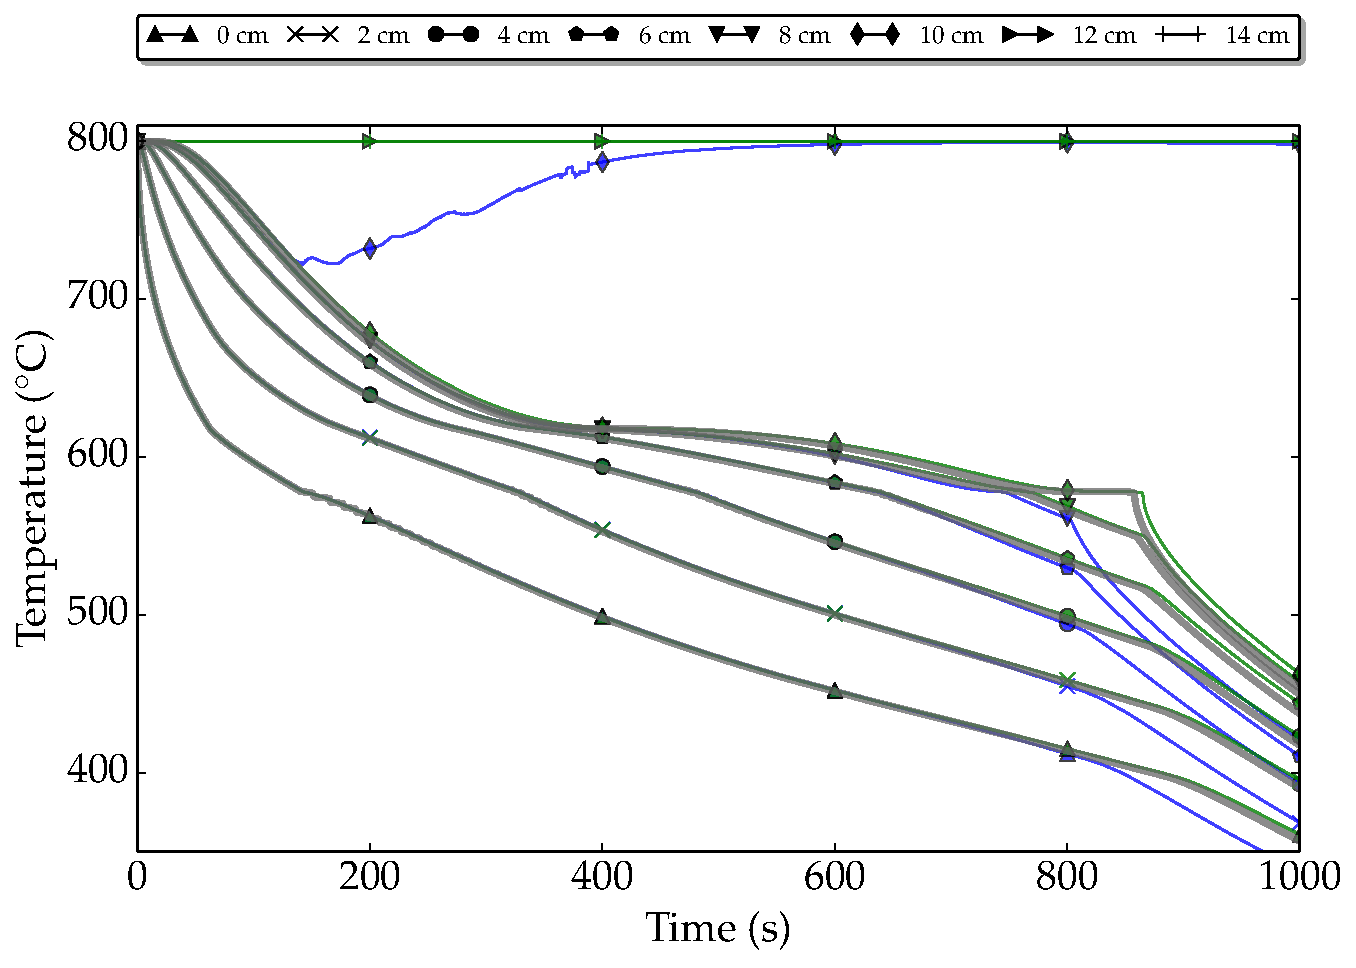
\includegraphics[width=\textwidth]{Chapter4/Data/1d_alsi7_cc/shrinkage_effect.pdf}
	\caption{Solidification shrinkage effect: grey curves correspond to a pure diffusion in a metal monodomain case,
			 \green{green} curves consider the latter case but with level set (metal and air subdomains) while \blue{blue} curves 
			 correspond to a shrinkage-driven flow case. All cases are solved without macrosegregation.}
    \label{fig:shrinkage_effect}
  \end{subfigure}
  %------------------------------
  \vskip\baselineskip
  %------------------------------
  \begin{subfigure}[t]{0.8\textwidth}
    \centering
	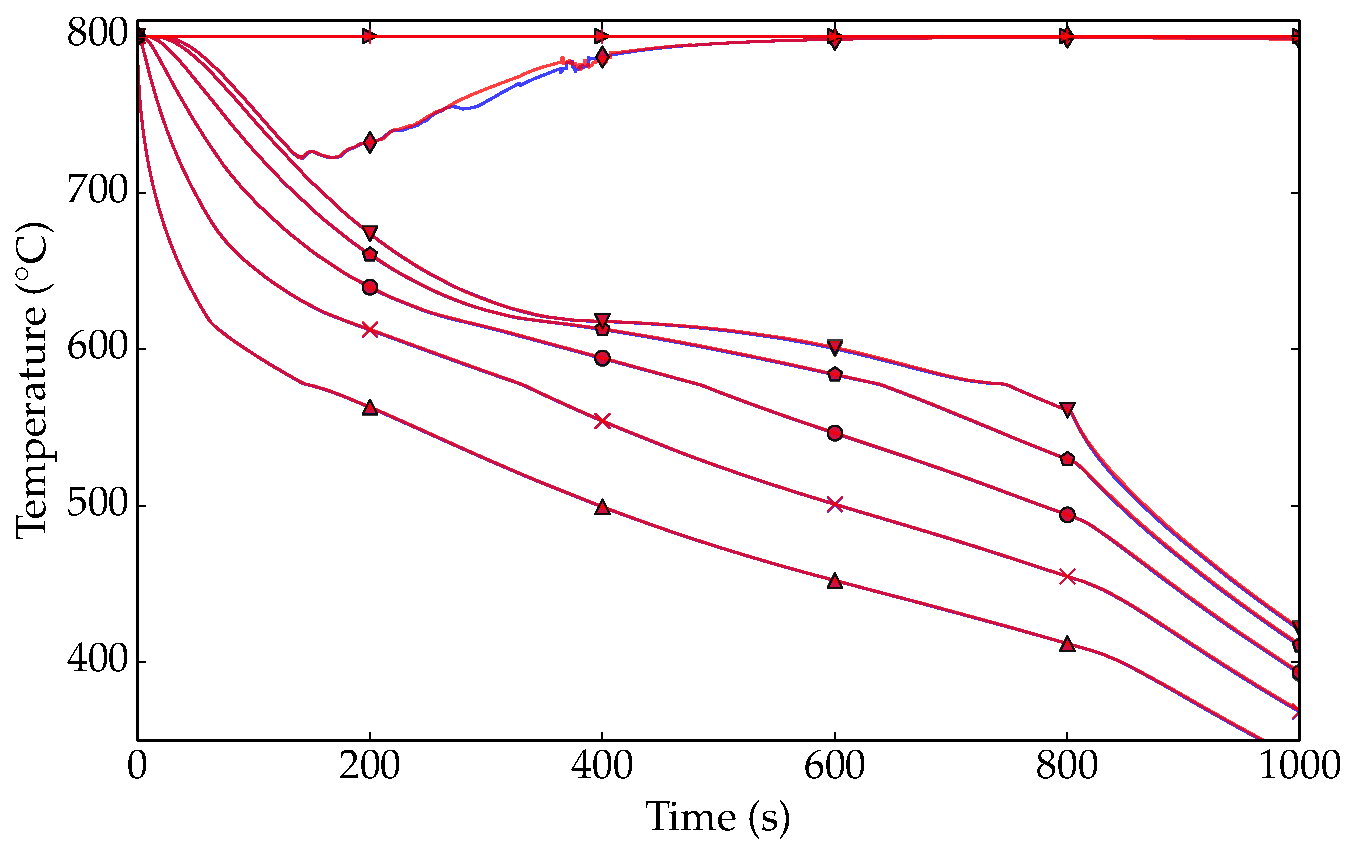
\includegraphics[width=\textwidth]{Chapter4/Data/1d_alsi7_cc/macro_effect.pdf}
	\caption{Macrosegregation effect: \blue{blue} curves represent the same simulation corresponding to the shrinkage-driven flow without macrosegregation, while
	the \red{red} curves correspond to a simulation of shrinkage-driven flow with macrosegregation.}
    \label{fig:macro_effect}
  \end{subfigure}
   %------------
\caption{Cooling curves at different fixed positions from 0 to 10 cm (intial metal length) and from 10 cm to 14 cm (initial air length) 
where we show (a) the effect of solidification shrinkage on temperature history without any macrosegregation then
we show (b) the effect of macrosegregation on temperature in the presence of solidification shrinkage.} 
\label{fig:1dasi7_macro_shrinkage}
\end{figure}
%------------------
%



%--------------
\begin{figureth}
% textwidth 
{1.0}
%path 
{Chapter4/Graphics/1d/macro/gs_w.pdf}
% caption
{My caption}
% label
\label{fig:somefig3}
\end{figureth}
%--------------





\section{2D application: \bin{Sn}{3}{Pb}}
Present 2D case with results + discussion

%--



\section{3D application: TEXUS steel}

\subsection{Introduction}
As presented in the introductory chapter, the aim of the CCEMLCC project is to "reach a better
understanding of surface defects formed during processing of steels from the liquid state" \citep{gandin_project_2014}.
Among the several scientific topics being studied, the interaction between skin macrosegregation 
and thermomechanical deformation is investigated through chill cooling experiments.
The idea is to have the molten steel in a containerless environment, which could be done by several ways: 
electromagnetic levitation, onboard parabolic flights or sounding rockets and finally
in a real microgravity context as in the ISS. Heat is extracted from the sample by contact with a ceramic 
(Si$_3$N$_4$) substrate at room temperature (hence the term "chill cooling"), that collides into the alloy at a controlled speed.
This contact situation generating high thermal gradients is comparable to casting processes between the molten alloy and the moulds.
For ground-based experiments, EML is the exclusive technique to achieve a chill cooling experiment. However, it is technically 
difficult to achieve levitation without currents in the spherical sample, generated by means of electromagnetic stirring (Lorentz forces) on the one hand but also
by thermal convection on the other hand. In reduced gravity conditions, the dynamics of the phenomena behind fluid motion are less significant.
The current application is therefore dedicated to chill cooling experiments performed in sounding rockets with reduced gravitational forces ($\norm{\gravity}$=\SI{e-5}{\uacceleration}).

%--------------
\begin{figureth}
% textwidth 
{1.0}
%path 
{Chapter4/Graphics/3d/exp.pdf}
% caption
{My caption}
% label
\label{fig:somefig2}
\end{figureth}
%--------------


\subsection{TEXUS experiment}
TEXUS-46 is actually the name of the sounding rocket that carries the experimental setup, 
but for simplicity we will refer to the latter as being the TEXUS experiment.



%--------------
\begin{figureth}
% textwidth 
{1.0}
%path 
{Chapter4/Graphics/3d/camera.pdf}
% caption
{Image sequence given by a high speed camera onboard a TEMPUS parabolic flight, showing the 
solidification progress between 0 s (when contact with the chill is initiated) to 3.75 s in a \tern{Fe}{0.9}{C}{0.2}{Si} steel droplet. 
The progress of the solidification front is marked by the green dashed line. In some frames, the droplet is partially hidden by the narrow 
opening of the sample holder facing the camera.}
% label
\label{fig:camera}
\end{figureth}
%--------------


\subsection{Previous contribution}
A former contribution by CEMEF was done by \citet{rivaux_simulation_2011}, as mentioned in the first chapter. 
His model considered both the steel droplet and the ceramic chill in a Lagrangian formulation, i.e. each object is
modelled using a separate deformable mesh. Conservation equations of mass, energy,
chemical species and momentum were solved in the metal domain, while the energy
conservation was the sole equation solved on the chill mesh. The mechanical problem was divided
into two parts: fluid and mechanics and solid mechanics. For the first part, the momentum conservation in the liquid phase was solved using an
incompressible P1/P1 SUPG-PSPG formulation of Navier-Stokes equations, i.e. without any contraction for the liquid phase neither solidification shrinkage at the solid-liquid interface.
The second part, solid mechanics,
was solved using P1+/P1 formulation to predict solid deformation caused by the previously mentioned factors, 
using elasto-visco-plastic behaviour. 
The simulation results showed that the total droplet deformation that has been
observed in the experiments is not primarily due to solid deformation. The density jump
between the solid and liquid phases at the solidification front is actually predominant. High
speed camera images endorse this observation, where the droplet underwent a continuous
spherical-to-elliptic shape change while the solidification front travelled away from the
contact point.
 
 
 
 
%--
